\section{Results: Indian Ocean tsunami}
\label{sec:results}
In this section, we compare the simulation results with recorded data of Indian Ocean tsunami. However, we do not compare the simulation results of the Japan tsunami. We that case study to demonstrate the performance.  
\subsection{Tidal gauge comparisons}
The numerical solutions are verified with the tide gauge records found in  \cite{gaugerecords}. Some of the previous work on validation using DGCOM \cite{gopalakrishnan2011tsunami} for Indian Ocean tsunami without a positivity preserving limiter is found in Alveras thesis \cite{alevras2009simulating}.

The important feature is the arrival time of the tsunami wave. The time at which the first peak in the elevation is observed, is considered to be the arrival time of a tsunami wave. Fig (\ref{fig:gauge_compare}), compares the simulation results with tidal gauge measurements at Chennai, Tuticorin, Mormugao, and Okha stations in India. The numerical model predicts the arrival times very accurately while the time history of the fluid heights estimated does not match the records exactly. 
\begin{figure}%[h!]
\begin{center}
  \subfloat[Chennai ($80.30^0 E$, $13.10^0 N$)]{%
    \begin{minipage}[c]{0.45\linewidth}
      \centering%
      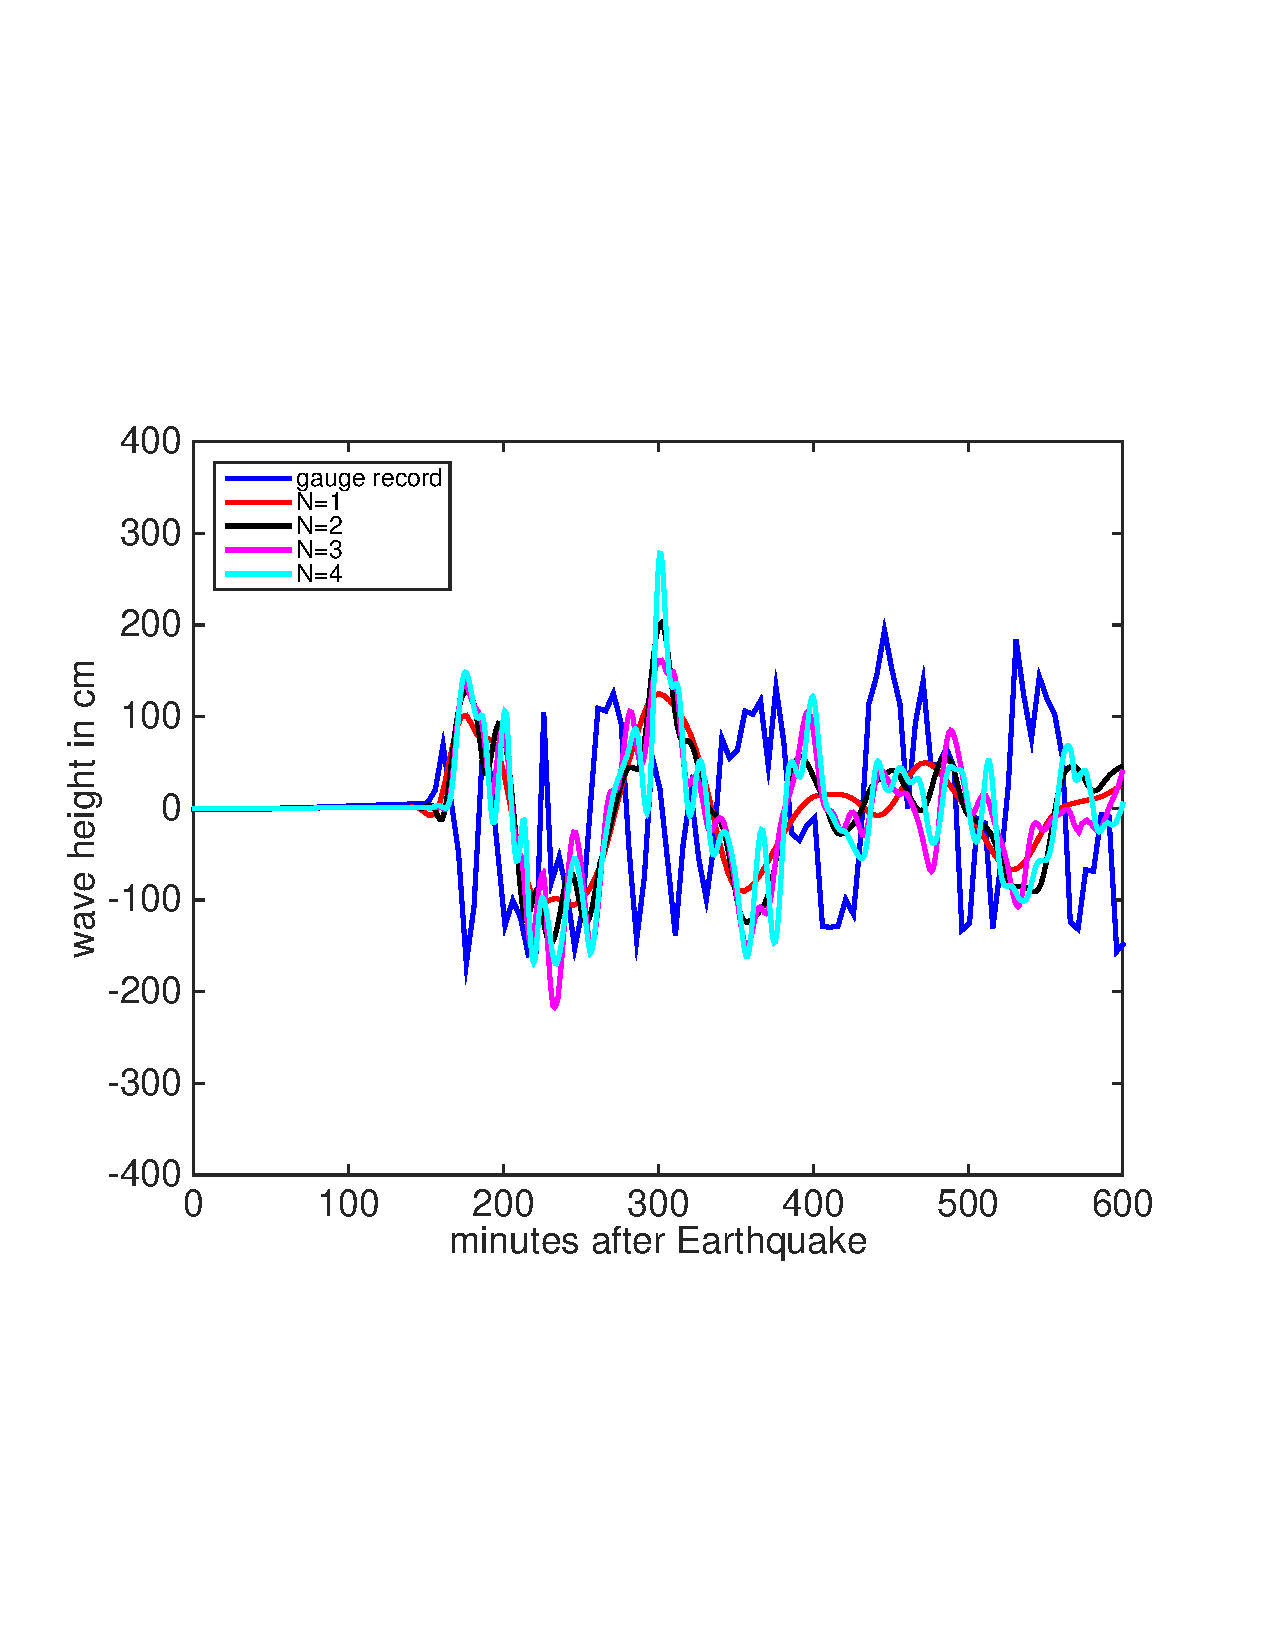
\includegraphics[trim=0cm 6cm 2cm 7cm,clip=true,width=\textwidth]{./figures/chennaiGaugeCon.pdf}
  \end{minipage}} \hspace{0.5cm}
  \subfloat[Tuticorin ($78.15^0 E$, $08.80^0 N$)]{%
    \begin{minipage}[c]{0.45\linewidth}
      \centering%
      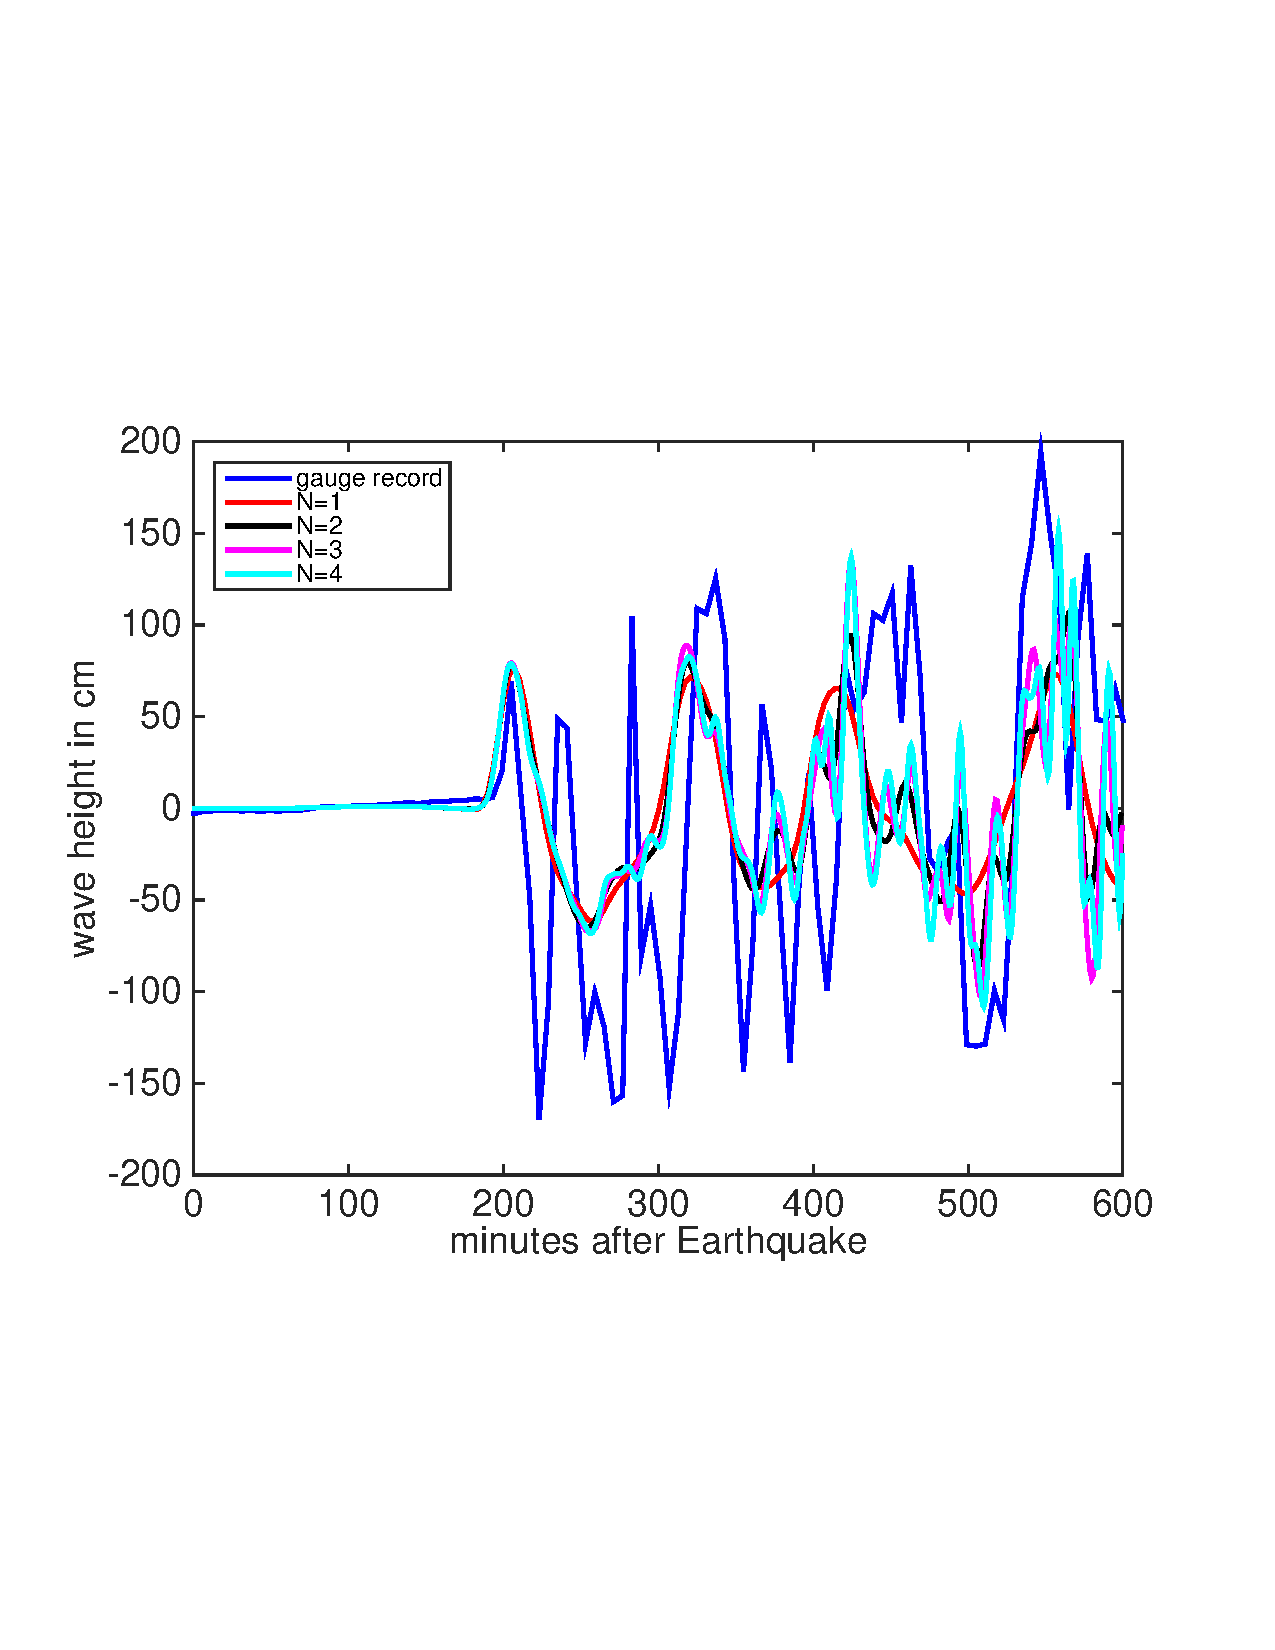
\includegraphics[trim=0cm 6cm 2cm 7cm,clip=true,width=\textwidth]{./figures/tuticorinGaugeCon.pdf}
  \end{minipage}}\\
    \subfloat[Mormugao ($73.80^0 E$, $15.42^0 N$)]{%
    \begin{minipage}[c]{0.45\linewidth}
      \centering%
      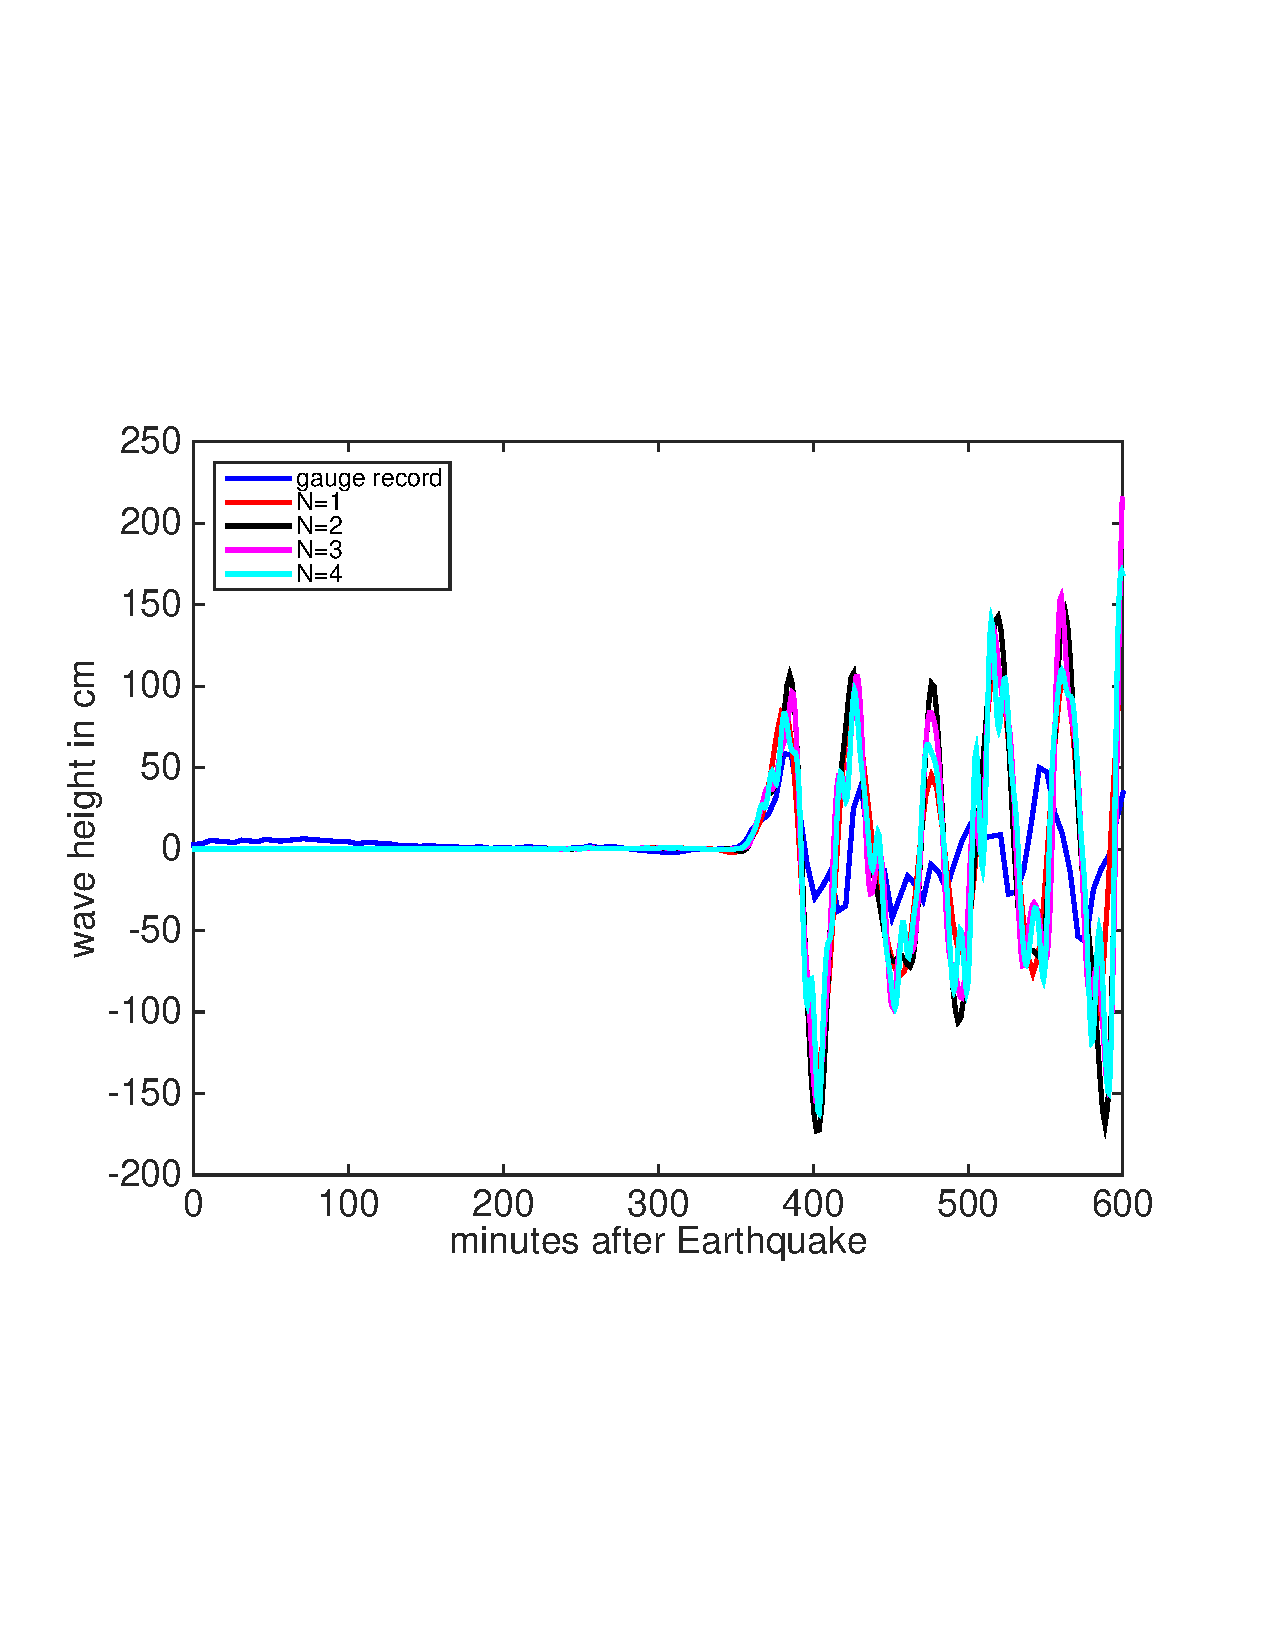
\includegraphics[trim=0cm 6cm 2cm 7cm,clip=true,width=\textwidth]{./figures/mormugaoGaugeCon.pdf}
  \end{minipage}} \hspace{0.5cm}
  \subfloat[Okha ($69.08^0 E$, $22.47^0 N$)]{%
    \begin{minipage}[c]{0.45\linewidth}
      \centering%
      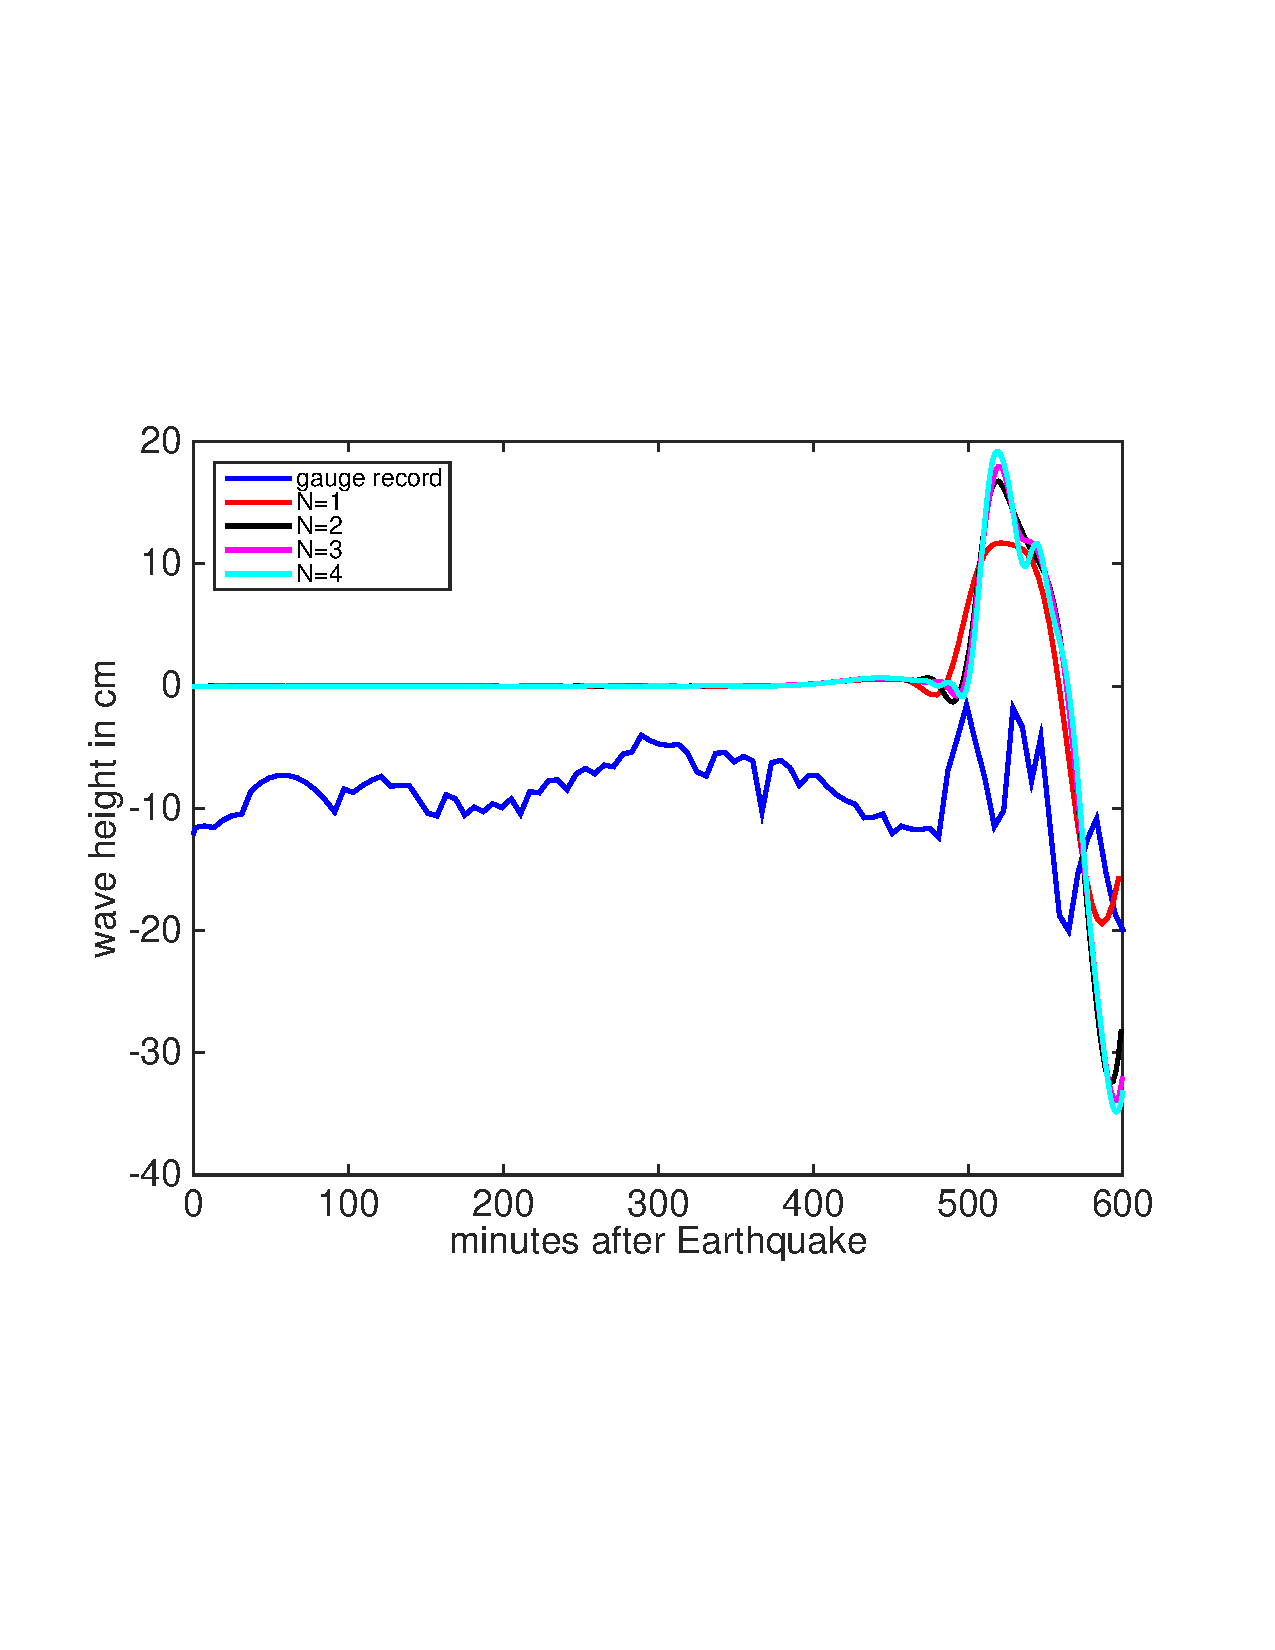
\includegraphics[trim=0cm 6cm 2cm 7cm,clip=true,width=\textwidth]{./figures/okhaGaugeCon.pdf}
  \end{minipage}}
\end{center}
 \caption{\emph{Comparison of simulation results with tidal gauge measurements at Chennai, Tuticorin, Mormugao, and Okha stations  in India.}}
  \label{fig:gauge_compare}
\end{figure}

\subsection{Fluid profile}
Fig (\ref{fig:tsunami_propagation}) shows the distribution of free surface elevation at $20$, $40$, $80$, and $160$ minutes after the Sumatra earthquake. These results are comparable with the results obtained  using ICOM \cite{pietrzak2007defining}.
In Fig (\ref{fig:tsunami_propagation_compare_N}), we show the free surface obtained at $80$ minutes using the simulation with approximation orders $1$ to $4$. These results are qualitatively similar. It might be due to the low resolution (linear in each triangle) of bathymetry distribution used.

\begin{figure}%[h!]
\begin{center}
  \subfloat[Free surface elevation at 20 min]{%
    \begin{minipage}[c]{0.35\linewidth}
      \centering%
      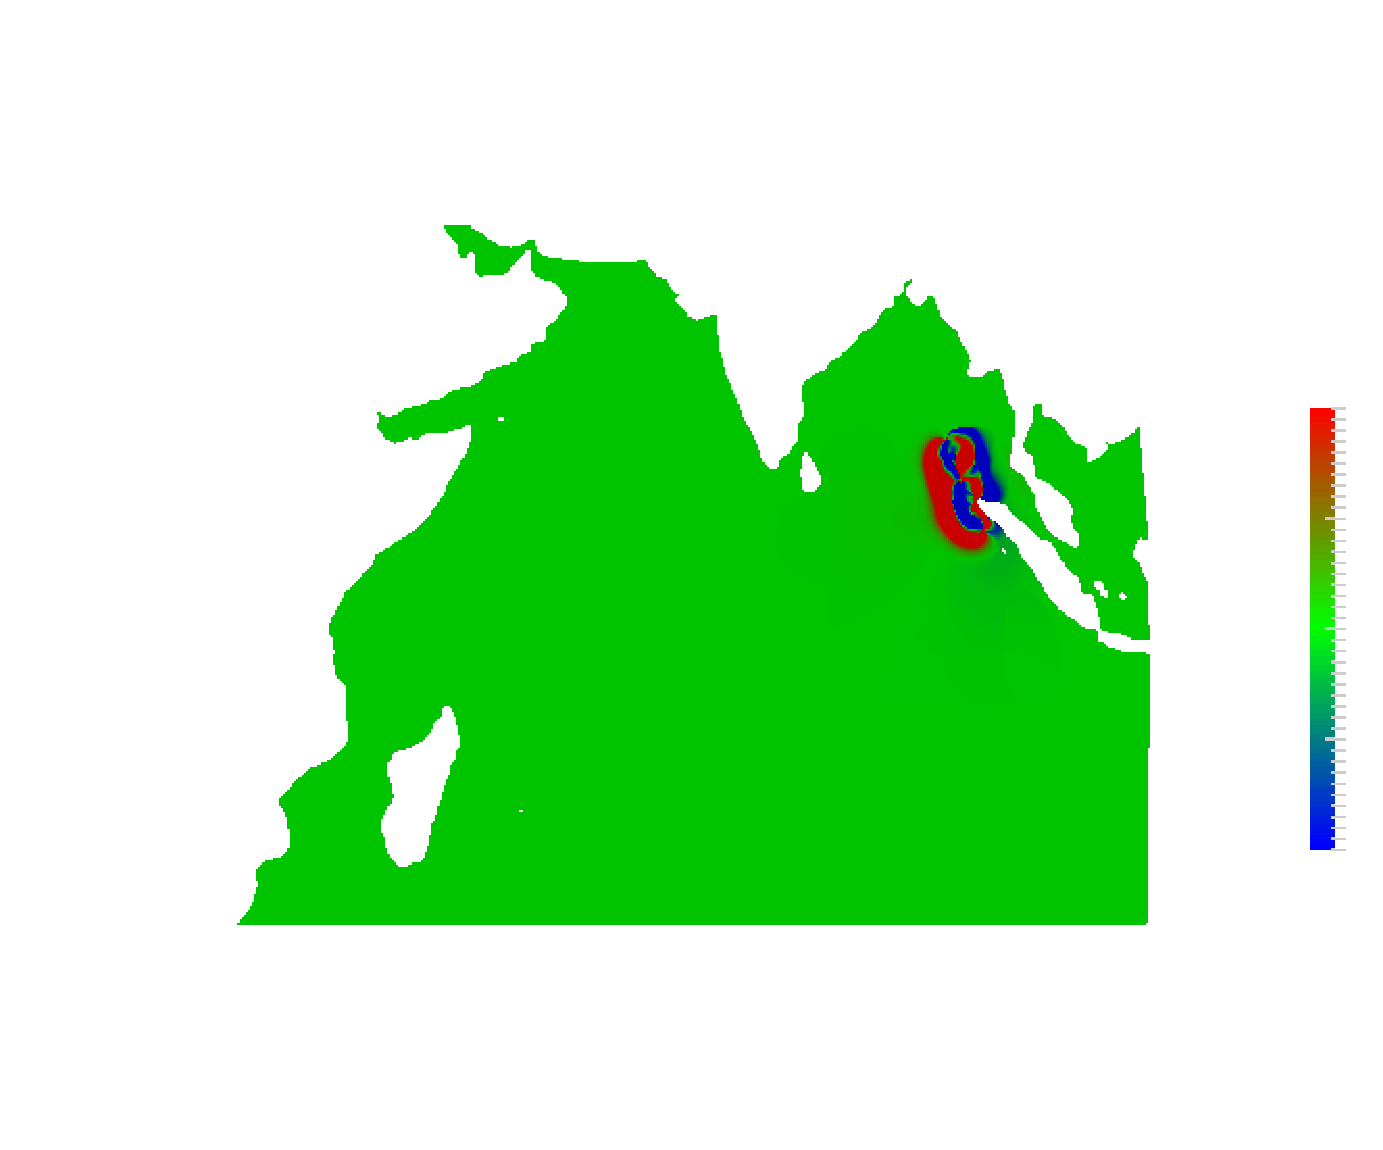
\includegraphics[trim=3.95cm 3.95cm 3.95cm 3.95cm,clip=true,width=\textwidth]{./figures/T20N4.pdf}
  \end{minipage}} \hspace{0.5cm}
  \subfloat[Free surface elevation at 40 min]{%
    \begin{minipage}[c]{0.35\linewidth}
      \centering%
      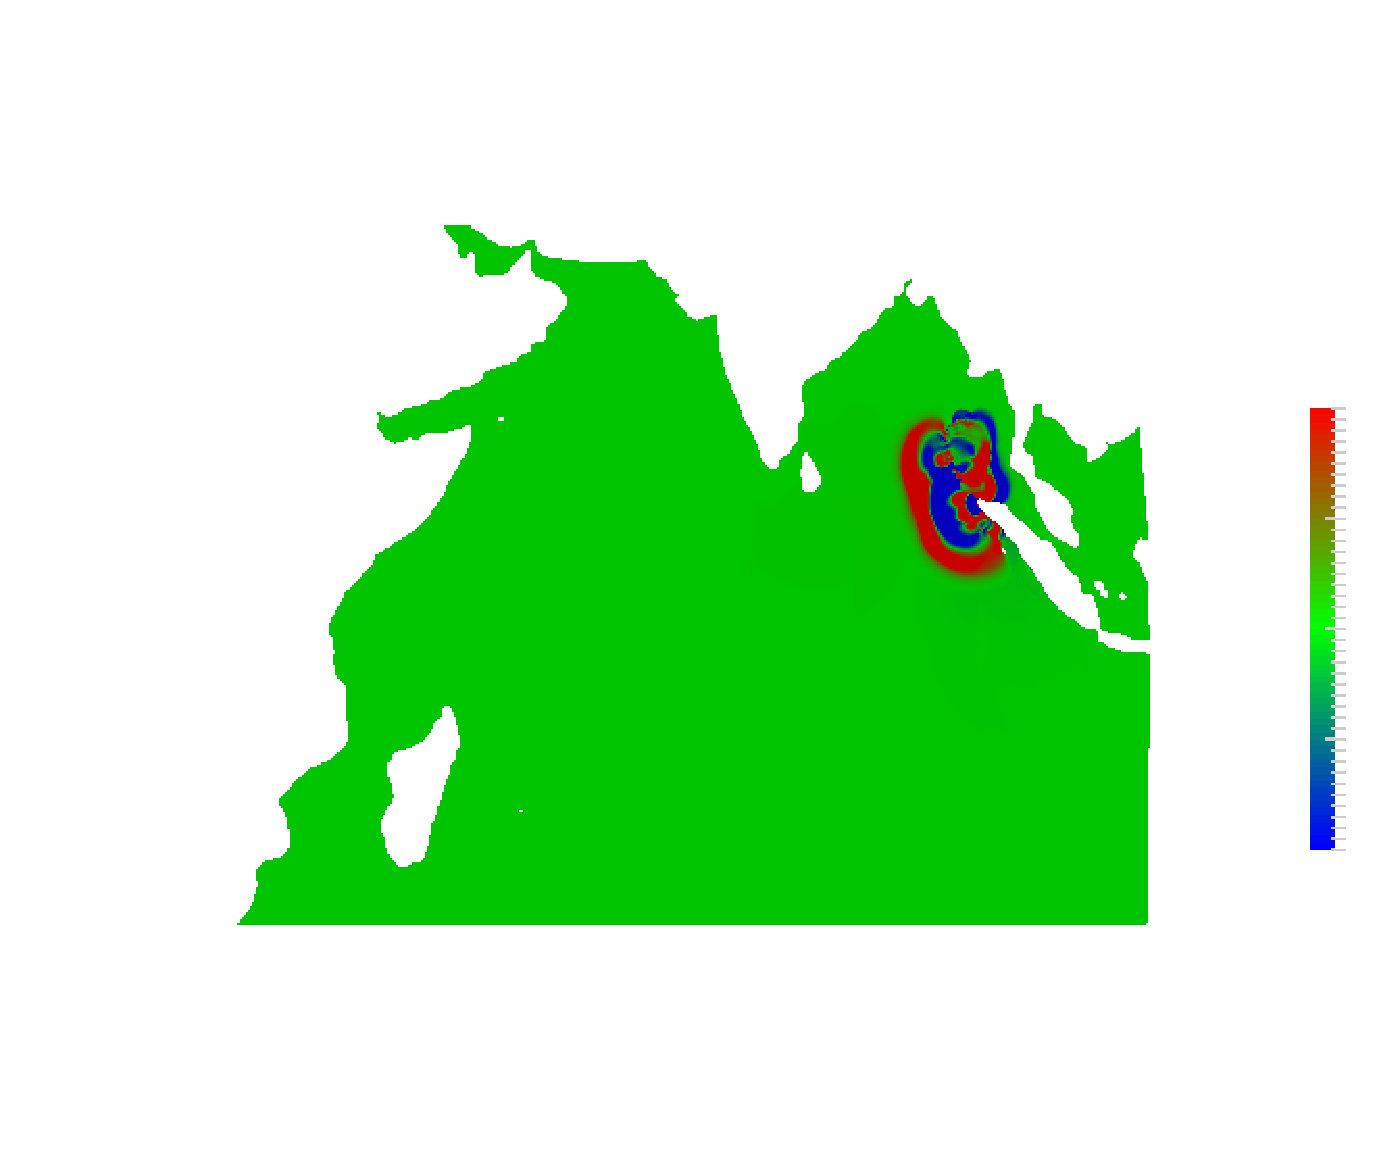
\includegraphics[trim=3.95cm 3.95cm 3.95cm 3.95cm,clip=true,width=\textwidth]{./figures/T40N4.pdf}
  \end{minipage}}\\
    \subfloat[Free surface elevation at 80 min]{%
    \begin{minipage}[c]{0.35\linewidth}
      \centering%
      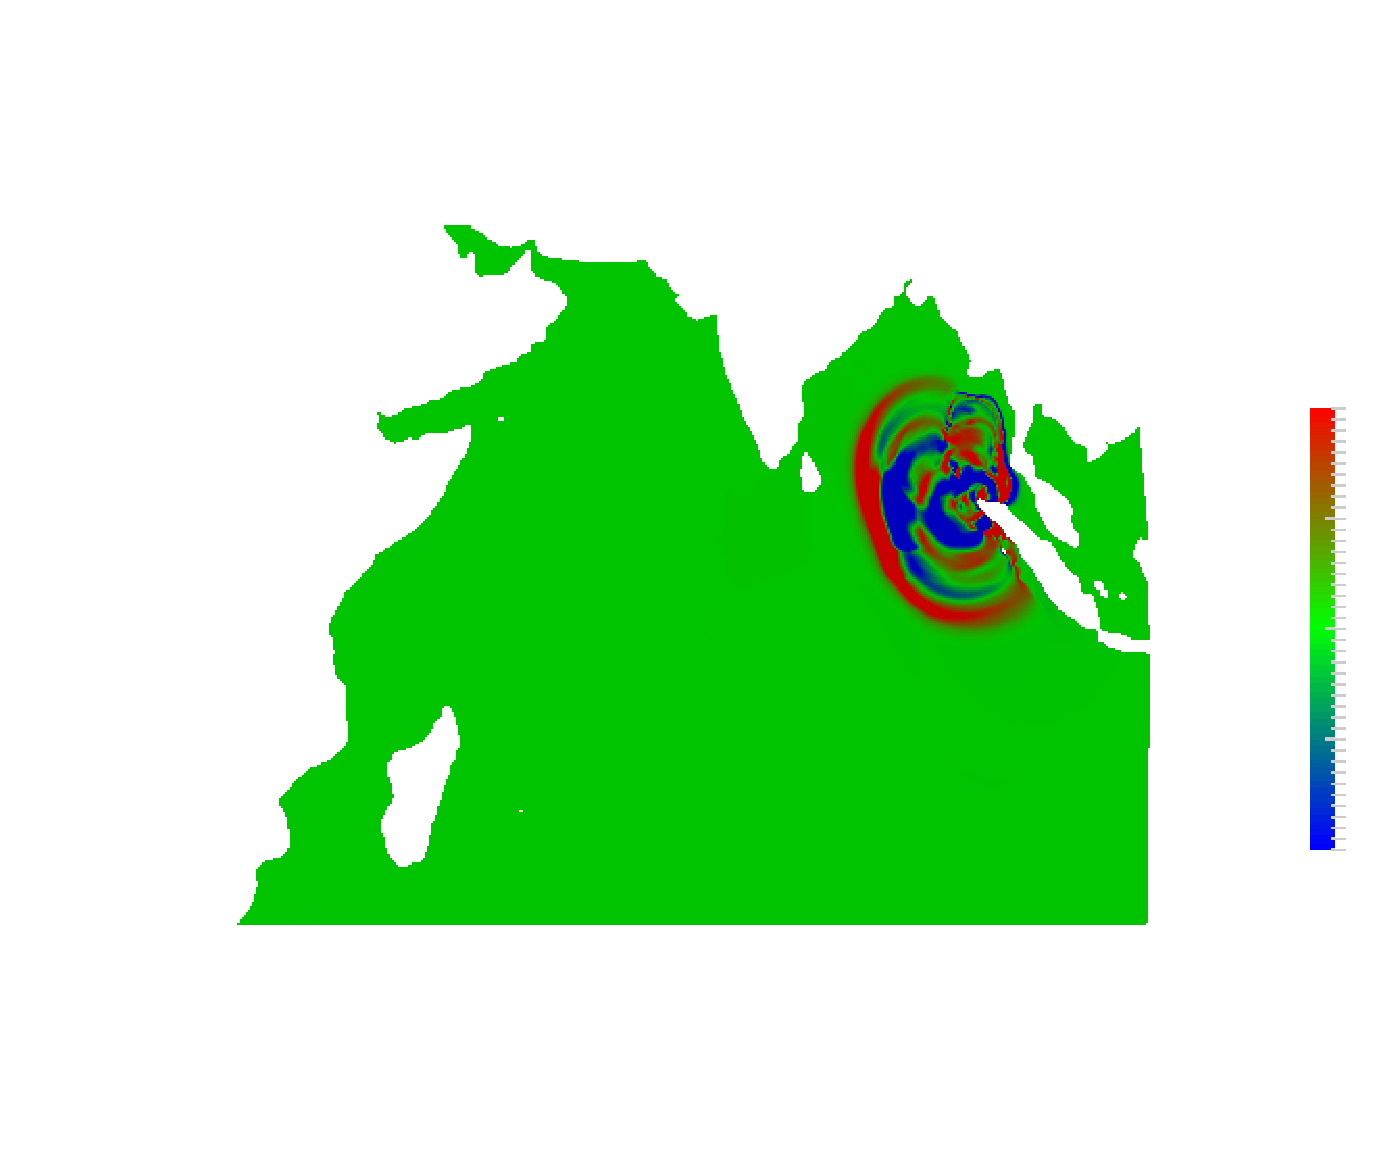
\includegraphics[trim=3.95cm 3.95cm 3.95cm 3.95cm,clip=true,width=\textwidth]{./figures/T80N4.pdf}
  \end{minipage}} \hspace{0.5cm}
  \subfloat[Free surface elevation at 160 min]{%
    \begin{minipage}[c]{0.35\linewidth}
      \centering%
      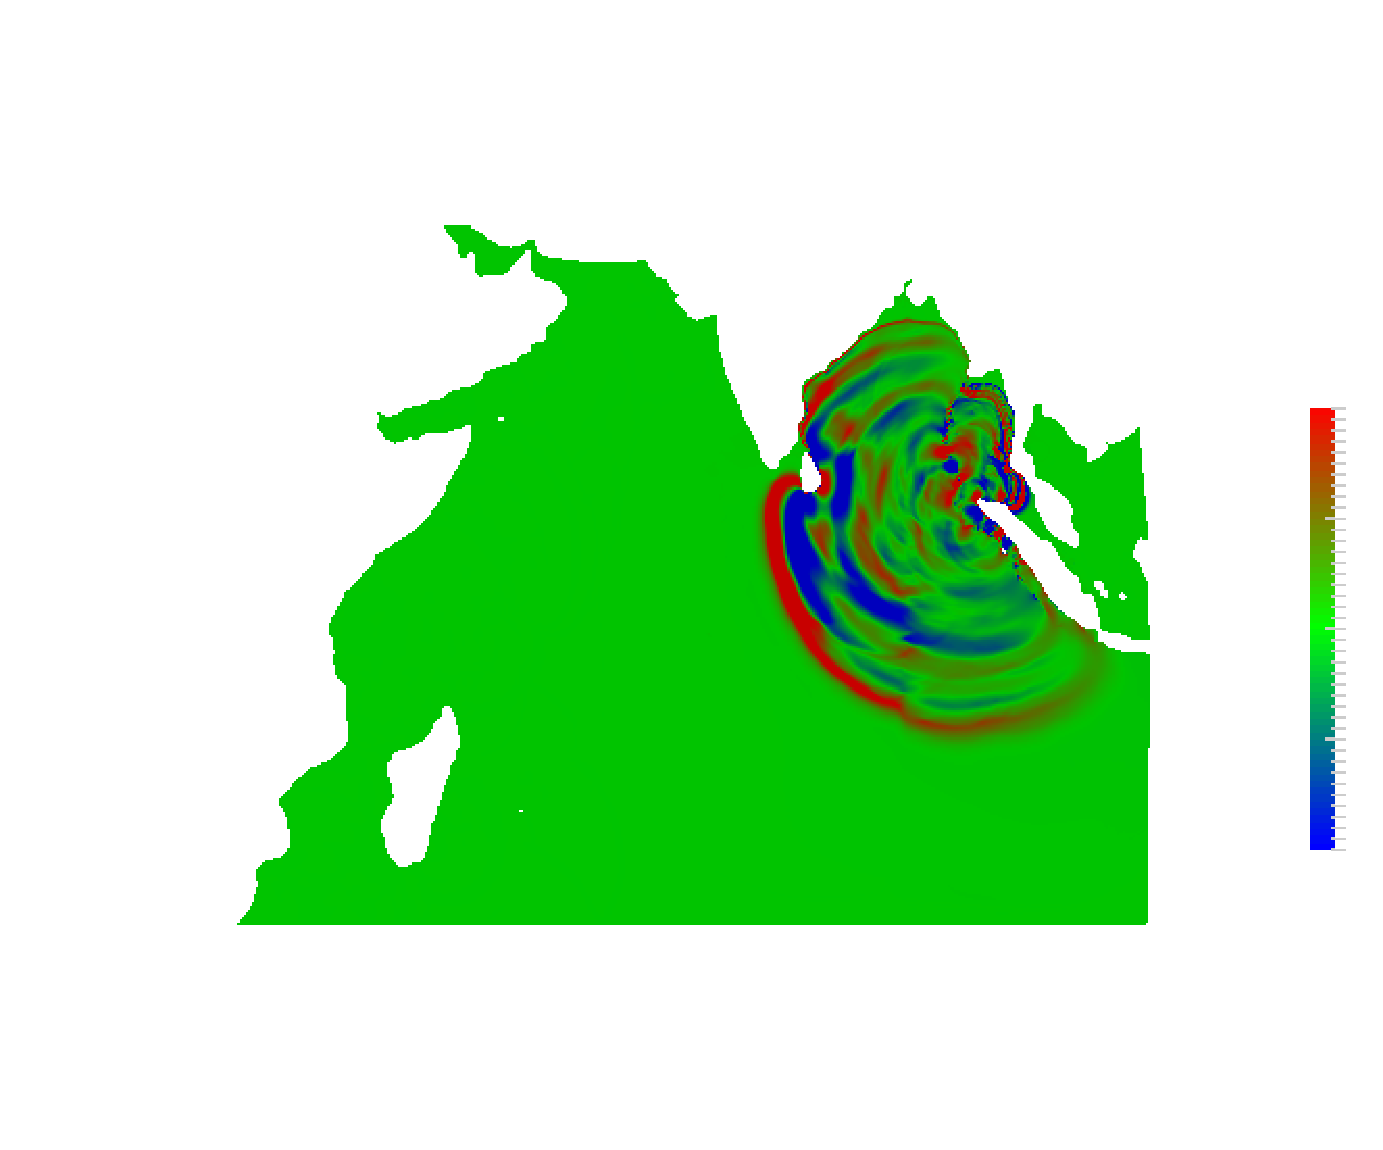
\includegraphics[trim=3.95cm 3.95cm 3.95cm 3.95cm,clip=true,width=\textwidth]{./figures/T160N4.pdf}
  \end{minipage}}\\
  \centering
   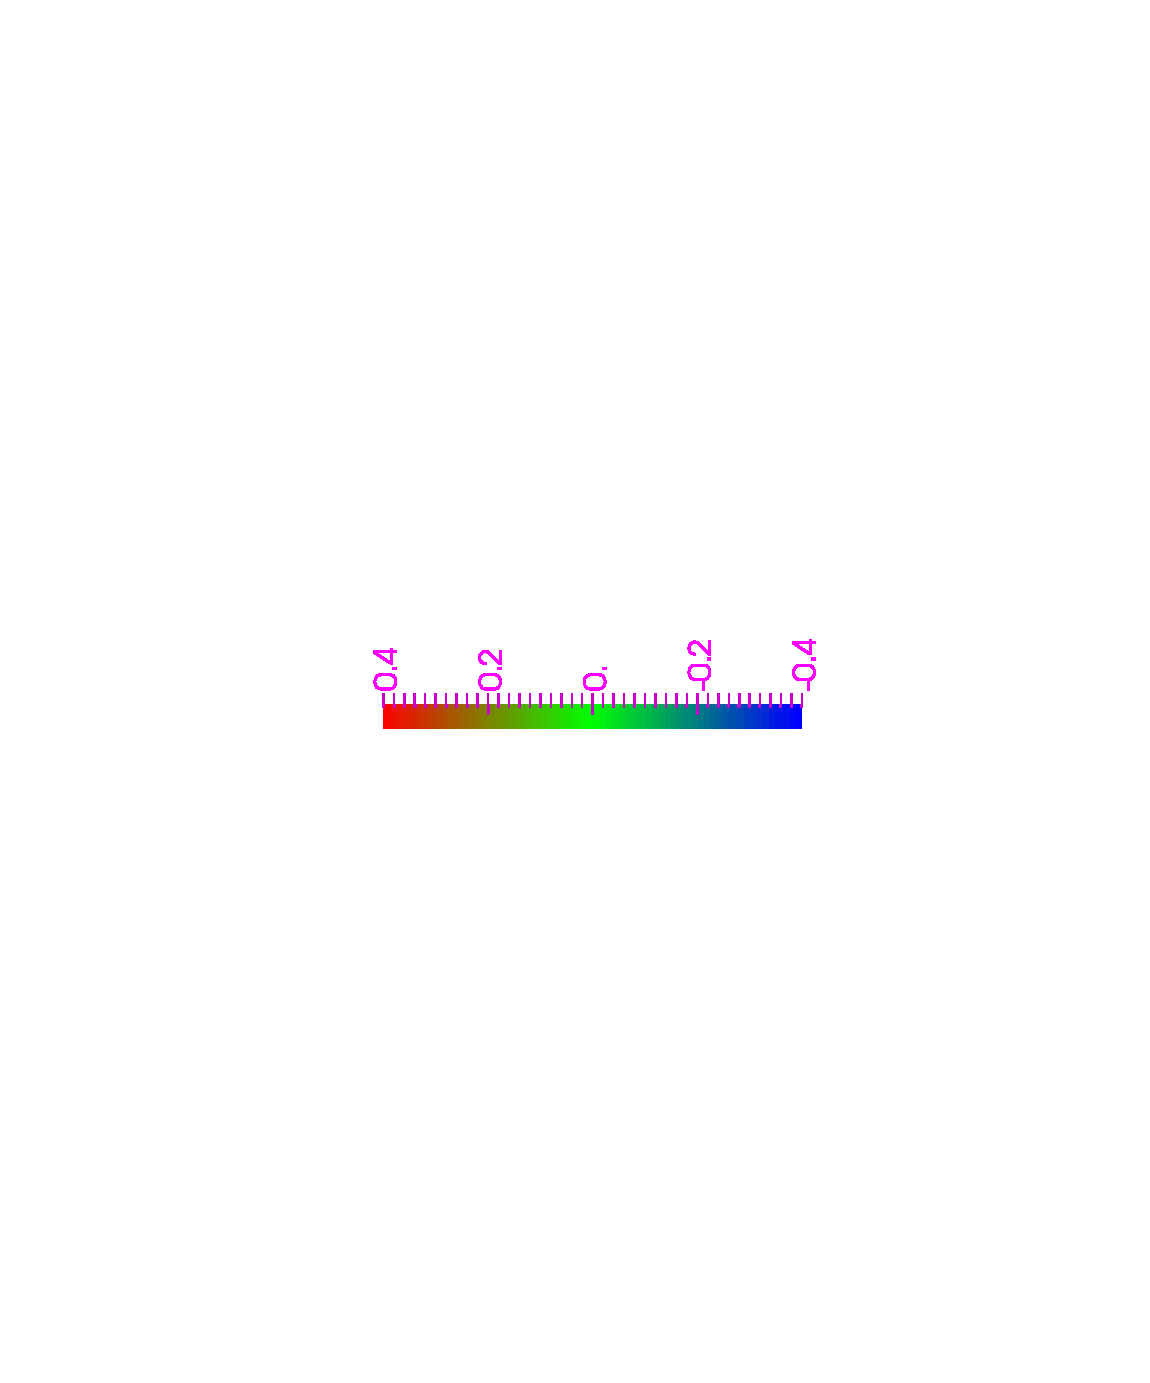
\includegraphics[trim=6cm 11cm 5cm 10.5cm,clip=true,width=0.5\textwidth]{./figures/TsunamiLegend.pdf}
\end{center}
 \caption{\emph{Free surface elevation of Indian Ocean tsunami at $20$, $40$,
$80$, and $160$ minutes after earthquake. Simulations are run with $4^{th}$
order polynomial approximation in each triangle with double precision arithmetic.}}
  \label{fig:tsunami_propagation}
\end{figure}

\begin{figure}%[h!]
\begin{center}
  \subfloat[N=1]{%
    \begin{minipage}[c]{0.45\linewidth}
      \centering%
      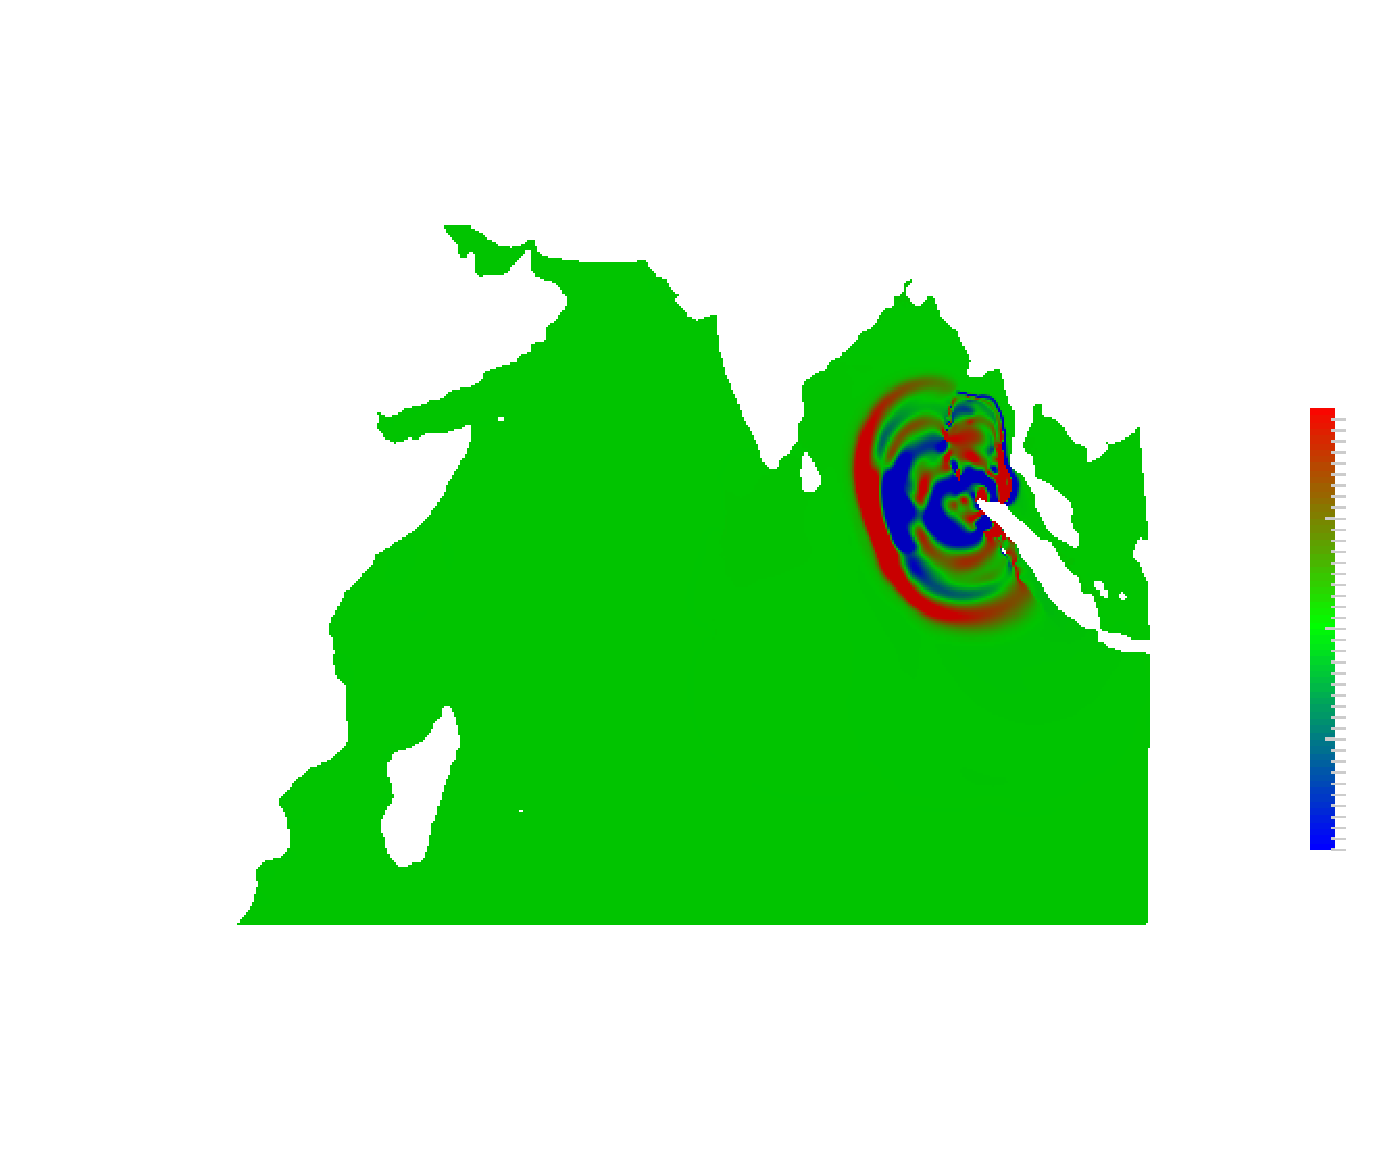
\includegraphics[trim=3.95cm 3.95cm 3.95cm 3.95cm,clip=true,width=\textwidth]{./figures/T80N1.pdf}
  \end{minipage}} \hspace{0.5cm}
  \subfloat[N=2]{%
    \begin{minipage}[c]{0.45\linewidth}
      \centering%
      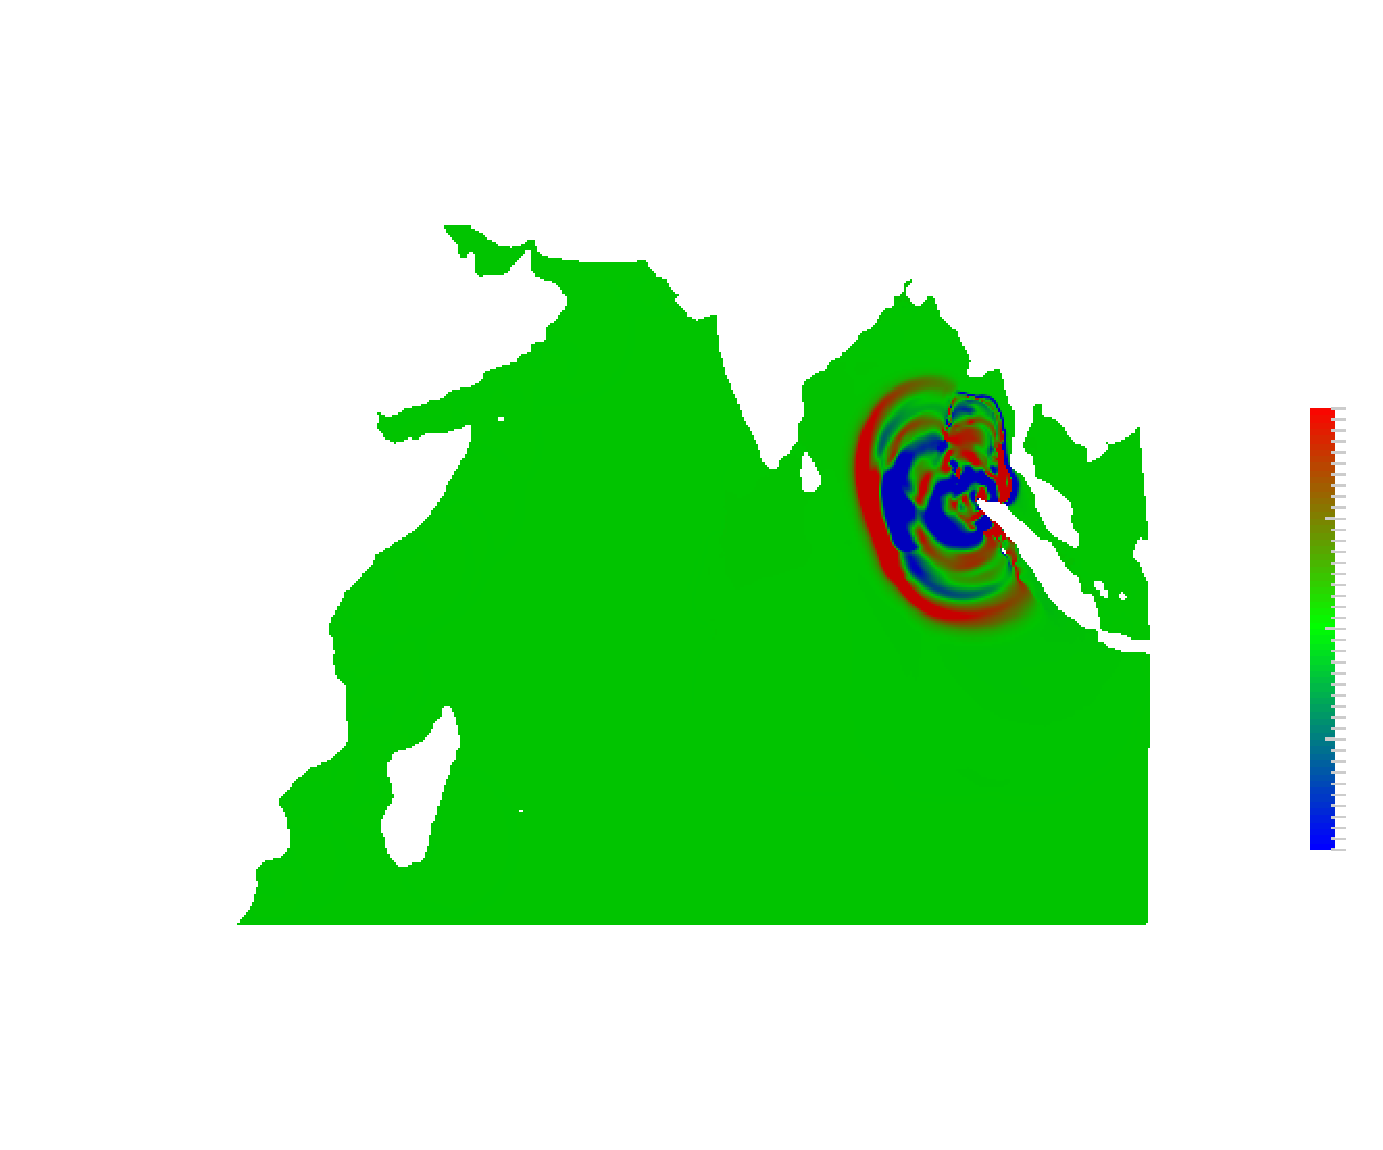
\includegraphics[trim=3.95cm 3.95cm 3.95cm 3.95cm,clip=true,width=\textwidth]{./figures/T80N2.pdf}
  \end{minipage}}\\
    \subfloat[N=3]{%
    \begin{minipage}[c]{0.45\linewidth}
      \centering%
      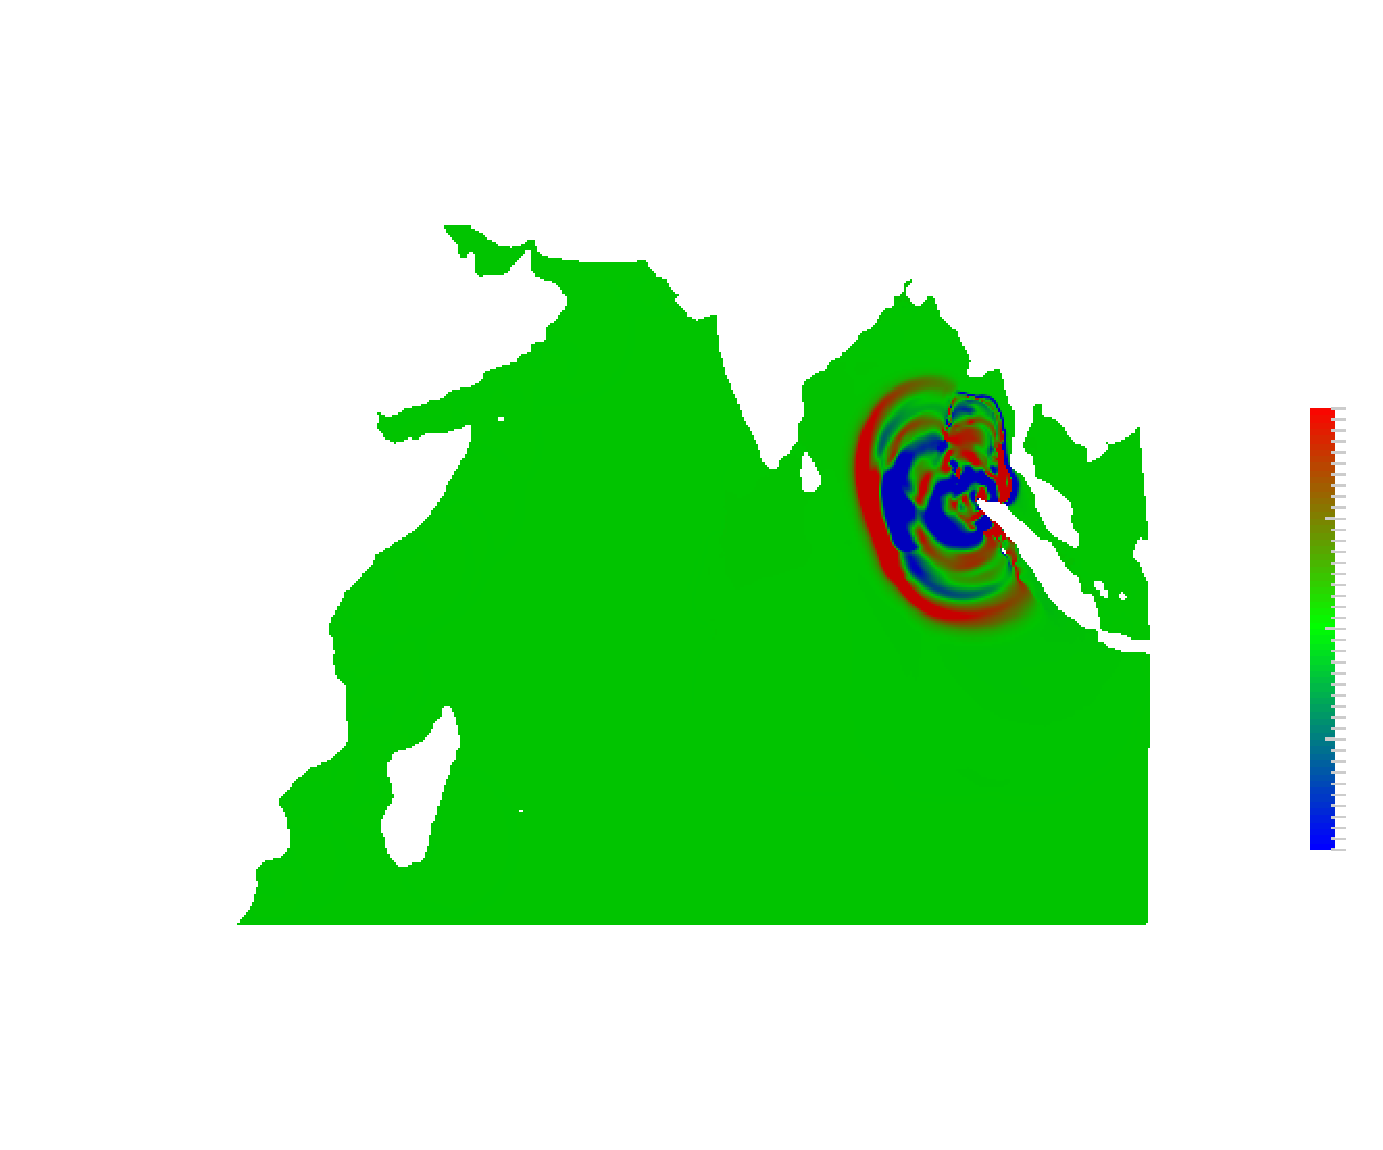
\includegraphics[trim=3.95cm 3.95cm 3.95cm 3.95cm,clip=true,width=\textwidth]{./figures/T80N3.pdf}
  \end{minipage}} \hspace{0.5cm}
  \subfloat[N=4]{%
    \begin{minipage}[c]{0.45\linewidth}
      \centering%
      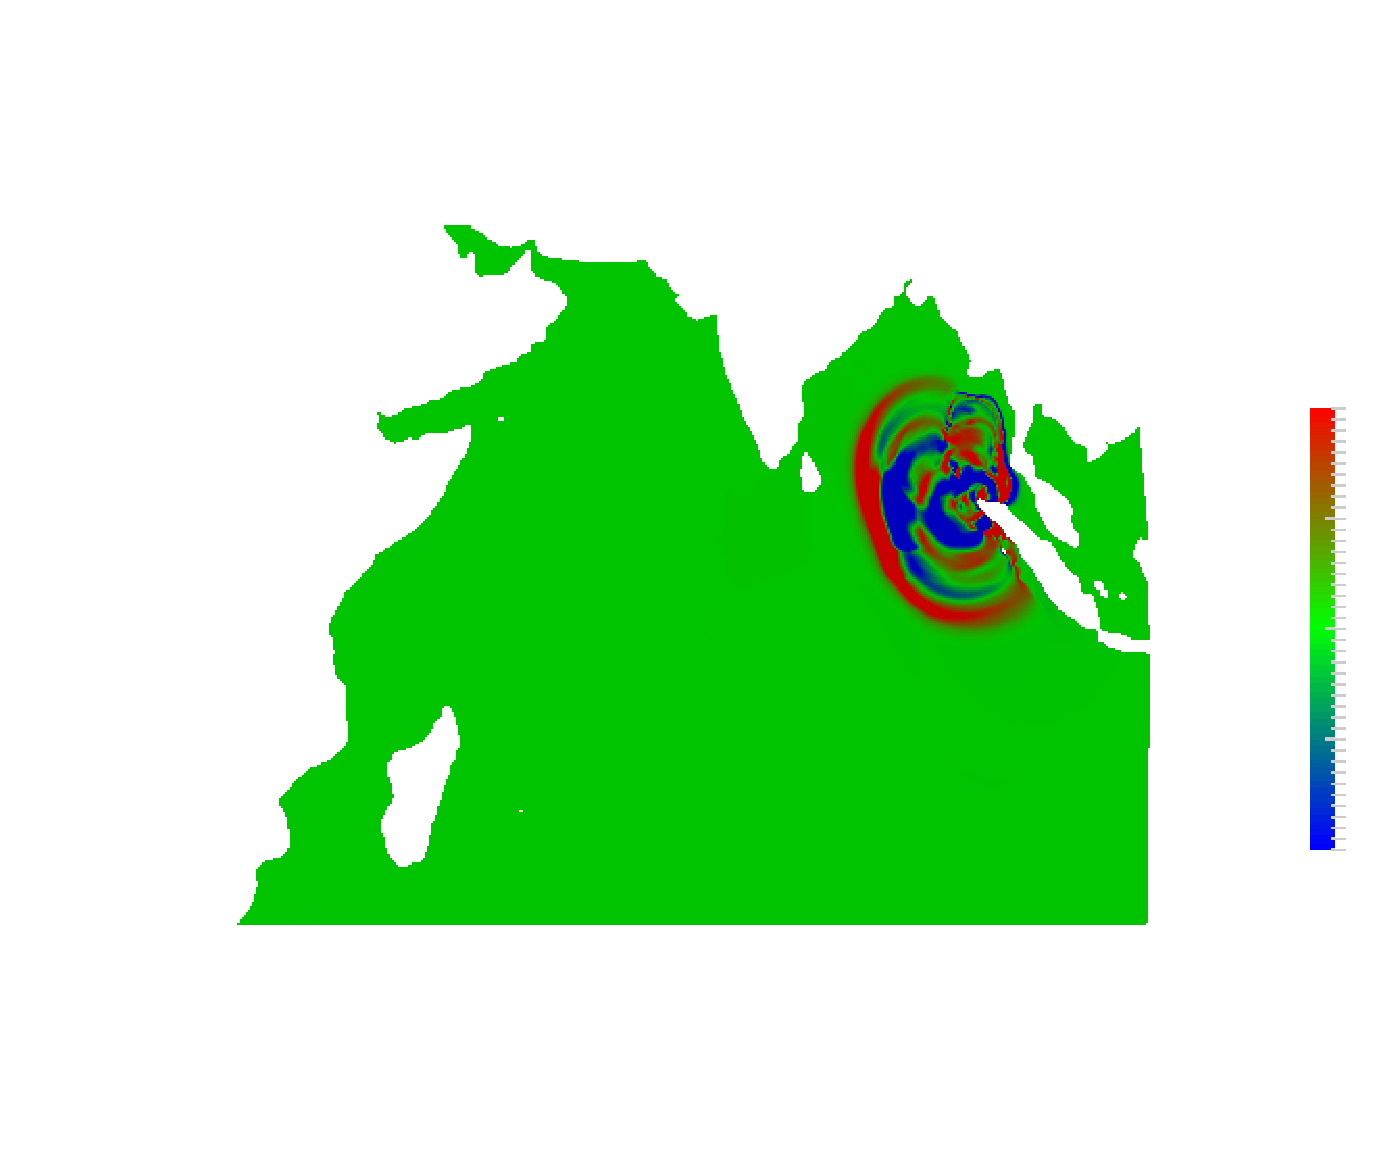
\includegraphics[trim=3.95cm 3.95cm 3.95cm 3.95cm,clip=true,width=\textwidth]{./figures/T80N4.pdf}
  \end{minipage}}\\
  \centering
   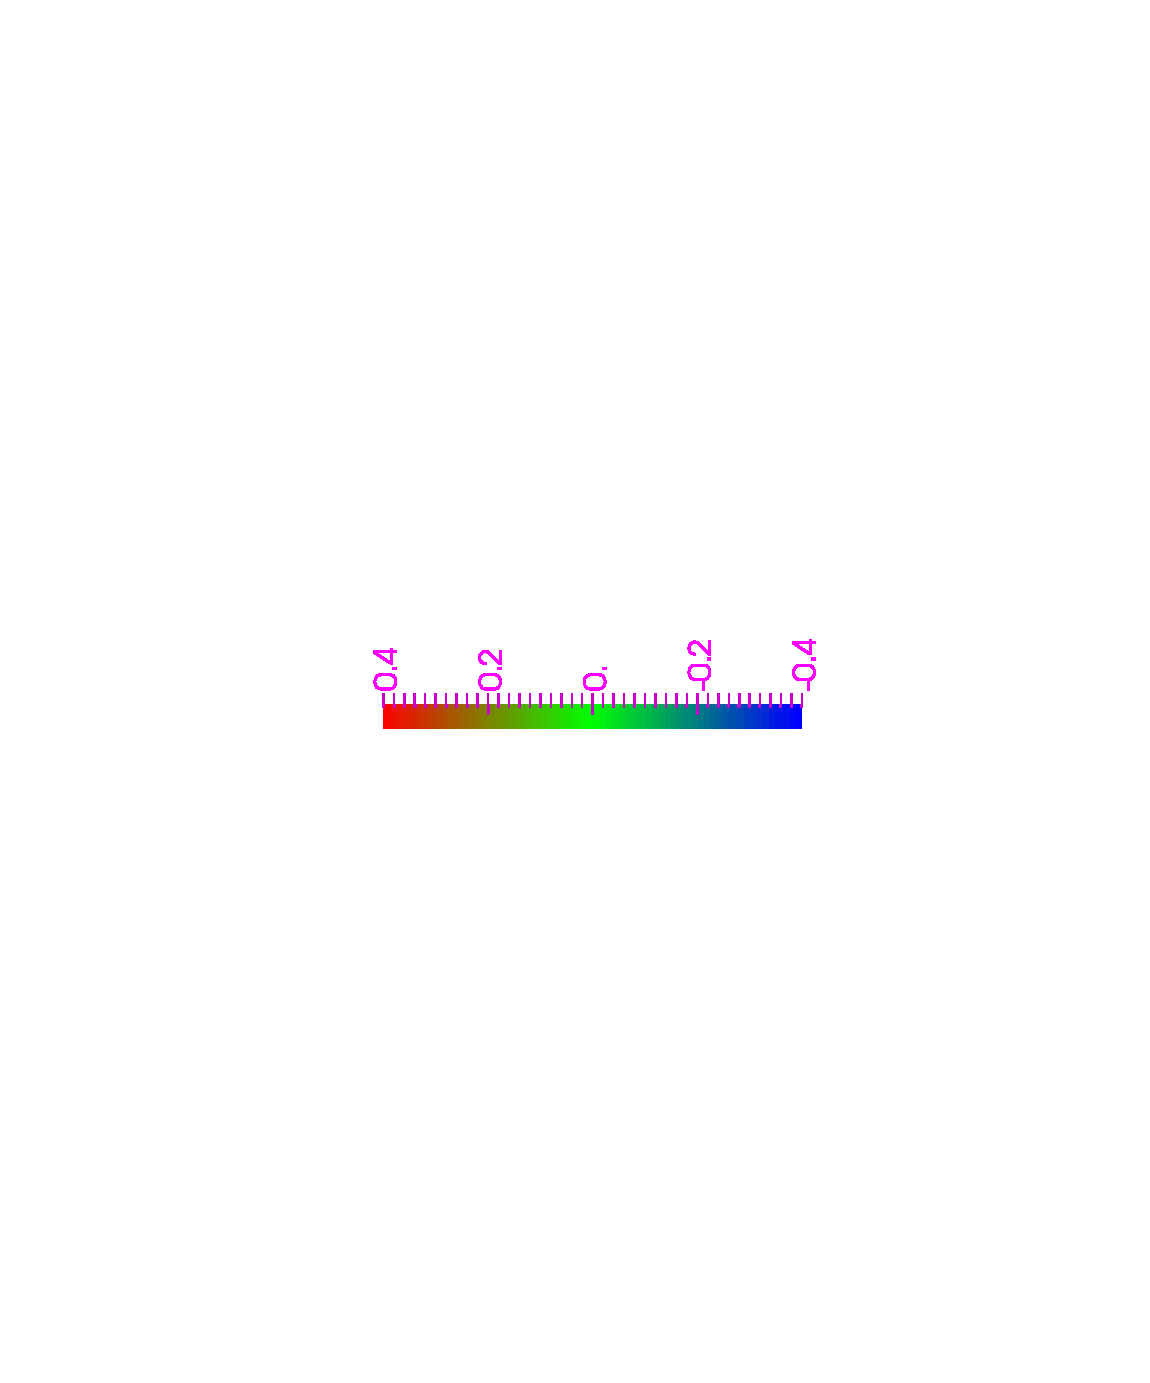
\includegraphics[trim=6cm 11cm 5cm 10.5cm,clip=true,width=0.5\textwidth]{./figures/TsunamiLegend.pdf}
\end{center}
 \caption{\emph{Free surface elevation of Indian Ocean tsunami at $80$ minutes
after earthquake. Simulations are run with $1$, $2$, $3$, and $4^{th}$ order
respectively.}}
  \label{fig:tsunami_propagation_compare_N}
\end{figure}


\subsection{Arrival time map}
One of the most important parameters in planning the evacuation in disaster management is the arrival time of the tsunamis. A surface plot of arrival time of the tsunami in the Indian Ocean and the coastal regions is shown in Fig (\ref{fig:arrivalTimeMap}). The arrival time is considered to be the time at which a free surface disturbance of $0.5m$ is observed for the first time. Using such arrival time maps, the critical regions can be identified during a real tsunami event. 
\begin{figure}[h!]
\begin{center}
%\centering
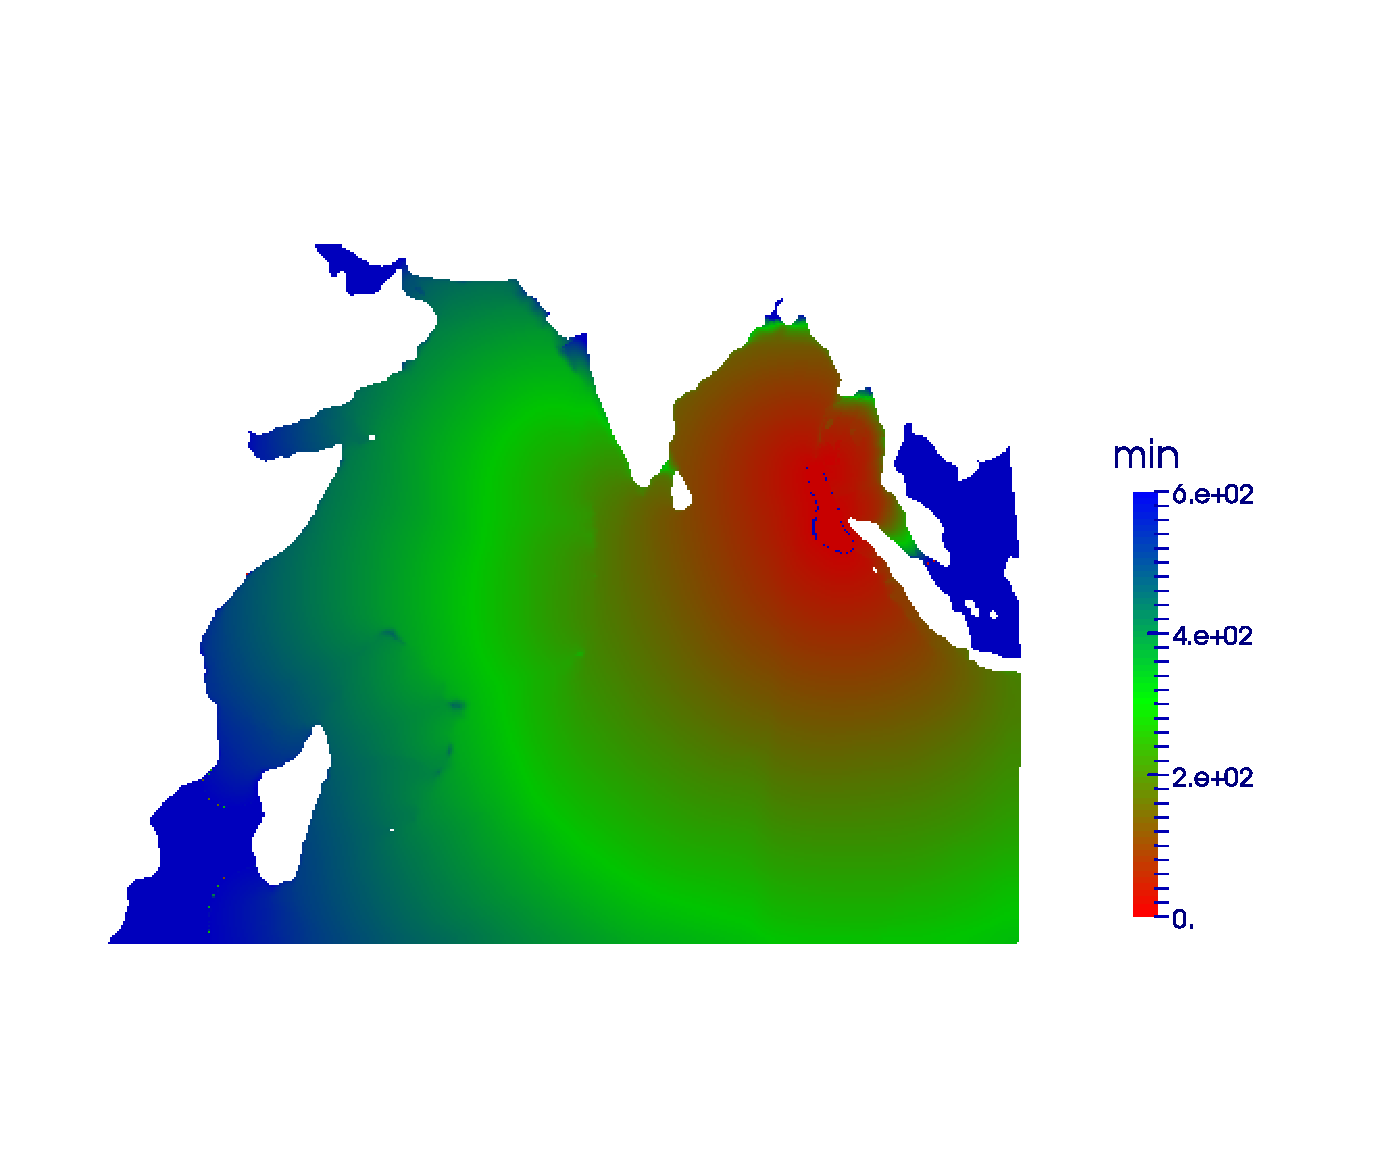
\includegraphics[trim=2cm 3cm 0cm 4cm,clip=true,width=0.5\linewidth]{./figures/arrivalTimeMapConN4.pdf}
\caption{\emph{Arrival time map in minutes. Simulations are ran using $4^{th}$ order polynomial representation in each triangle.}}
\label{fig:arrivalTimeMap}
\end{center}
\end{figure}

\subsection{Performance}
The performance of the kernels and efficiency of the overall solver with several threading models through the OCCA framework are presented in \cite{gandham2014swe} with the aid of analytical test cases. Here, the performance of the multi-rate scheme and overall solver for a realistic problem are presented. For the simulations, polynomial orders of $1$, $2$, $3$, and $4$ are considered.

Fig (\ref{fig:timeVsLevels}) shows the speedup achieved with multi-rate time stepping scheme with respect to the single rate scheme. The computational time required by the coarse elements decreases with the increase in number of levels. As a result, it is expected that the computational time decreases with the increasing number of levels used for the multi-rate scheme. However, the computations kernels are inefficient when the number of elements processed by the kernels is very low. Hence, there is no significant speedup when $4$ levels are used compared to when only $3$ levels are used for the simulation.  
\begin{figure}[h!]
\begin{center}
%\centering
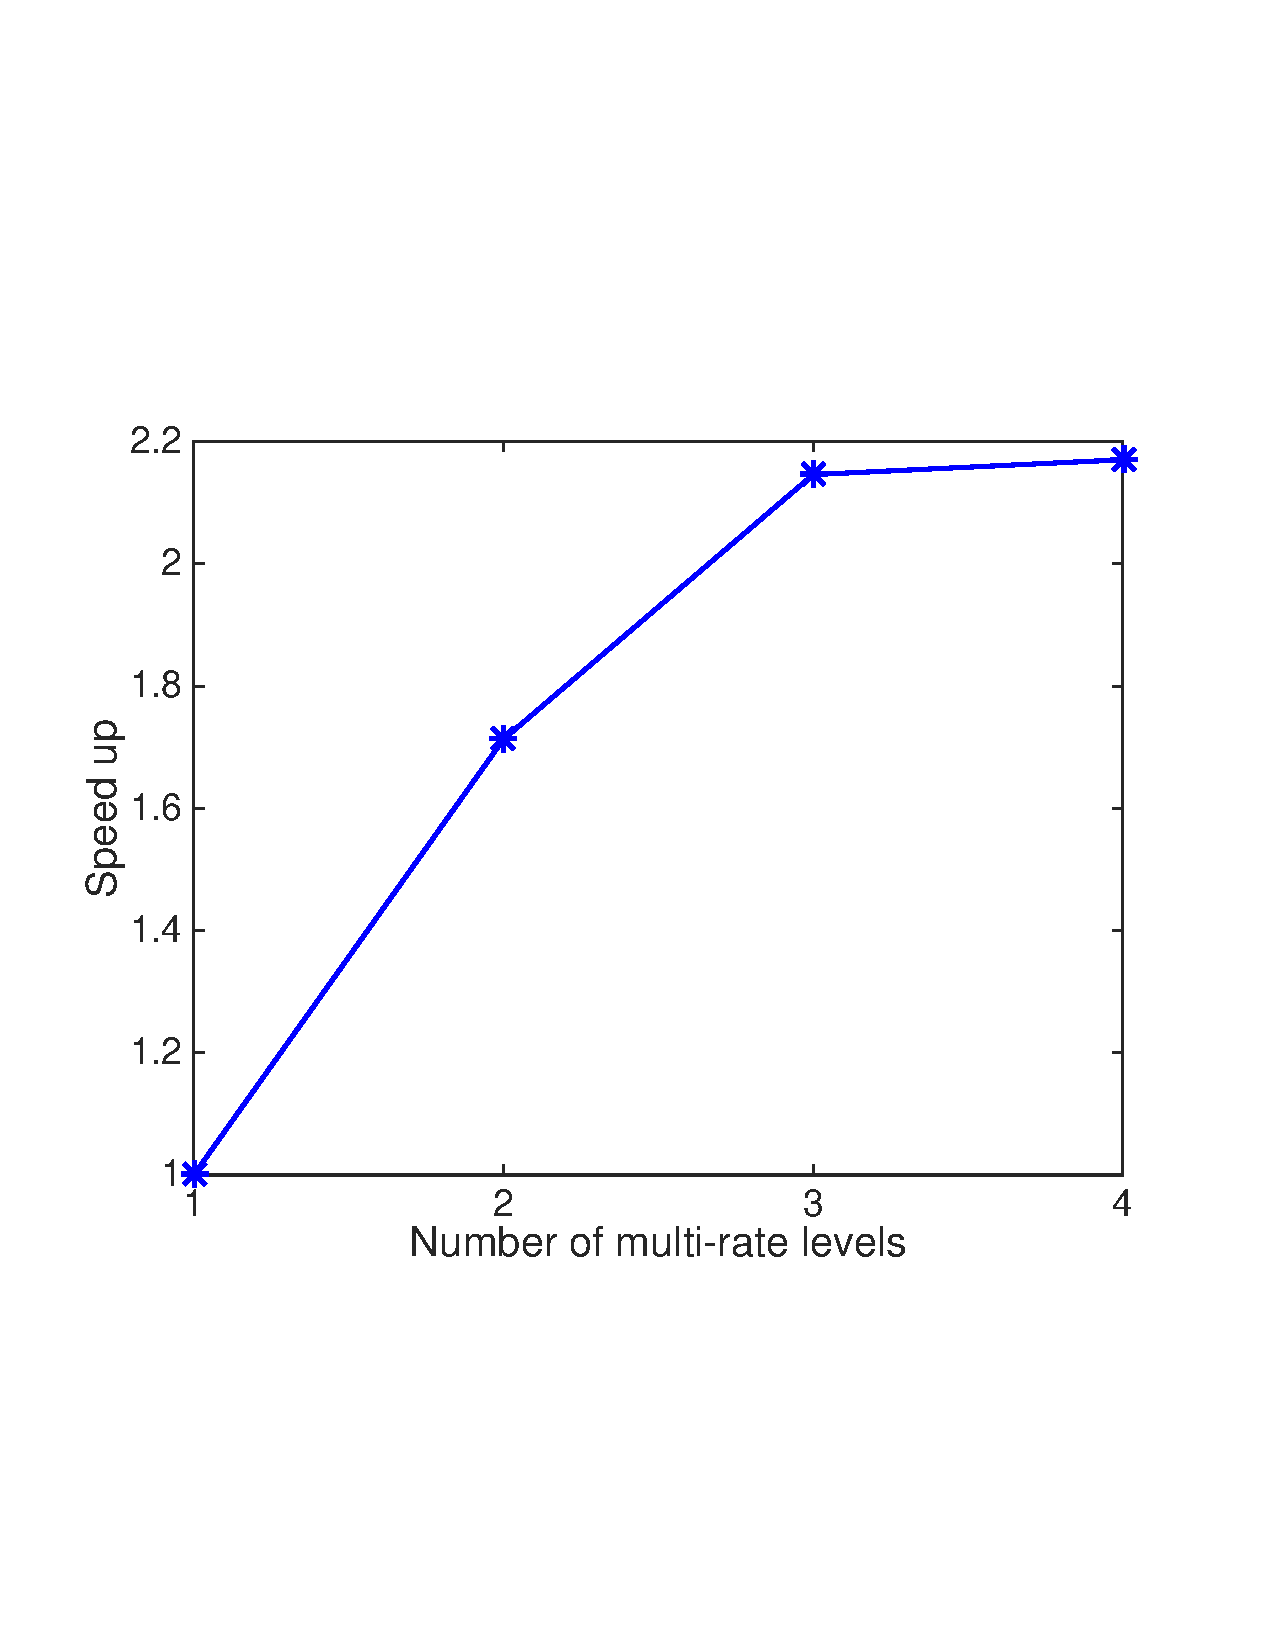
\includegraphics[trim=1cm 6cm 2cm 7cm,clip=true,width=0.5\linewidth]{./figures/timeVsLevels.pdf}
\caption{\emph{Overall speedup vs the number of multi-rate levels used for the simulation of Indian Ocean tsunami.}}
\label{fig:timeVsLevels}
\end{center}
\end{figure}

\begin{figure}[h!]
\begin{center}
%\centering
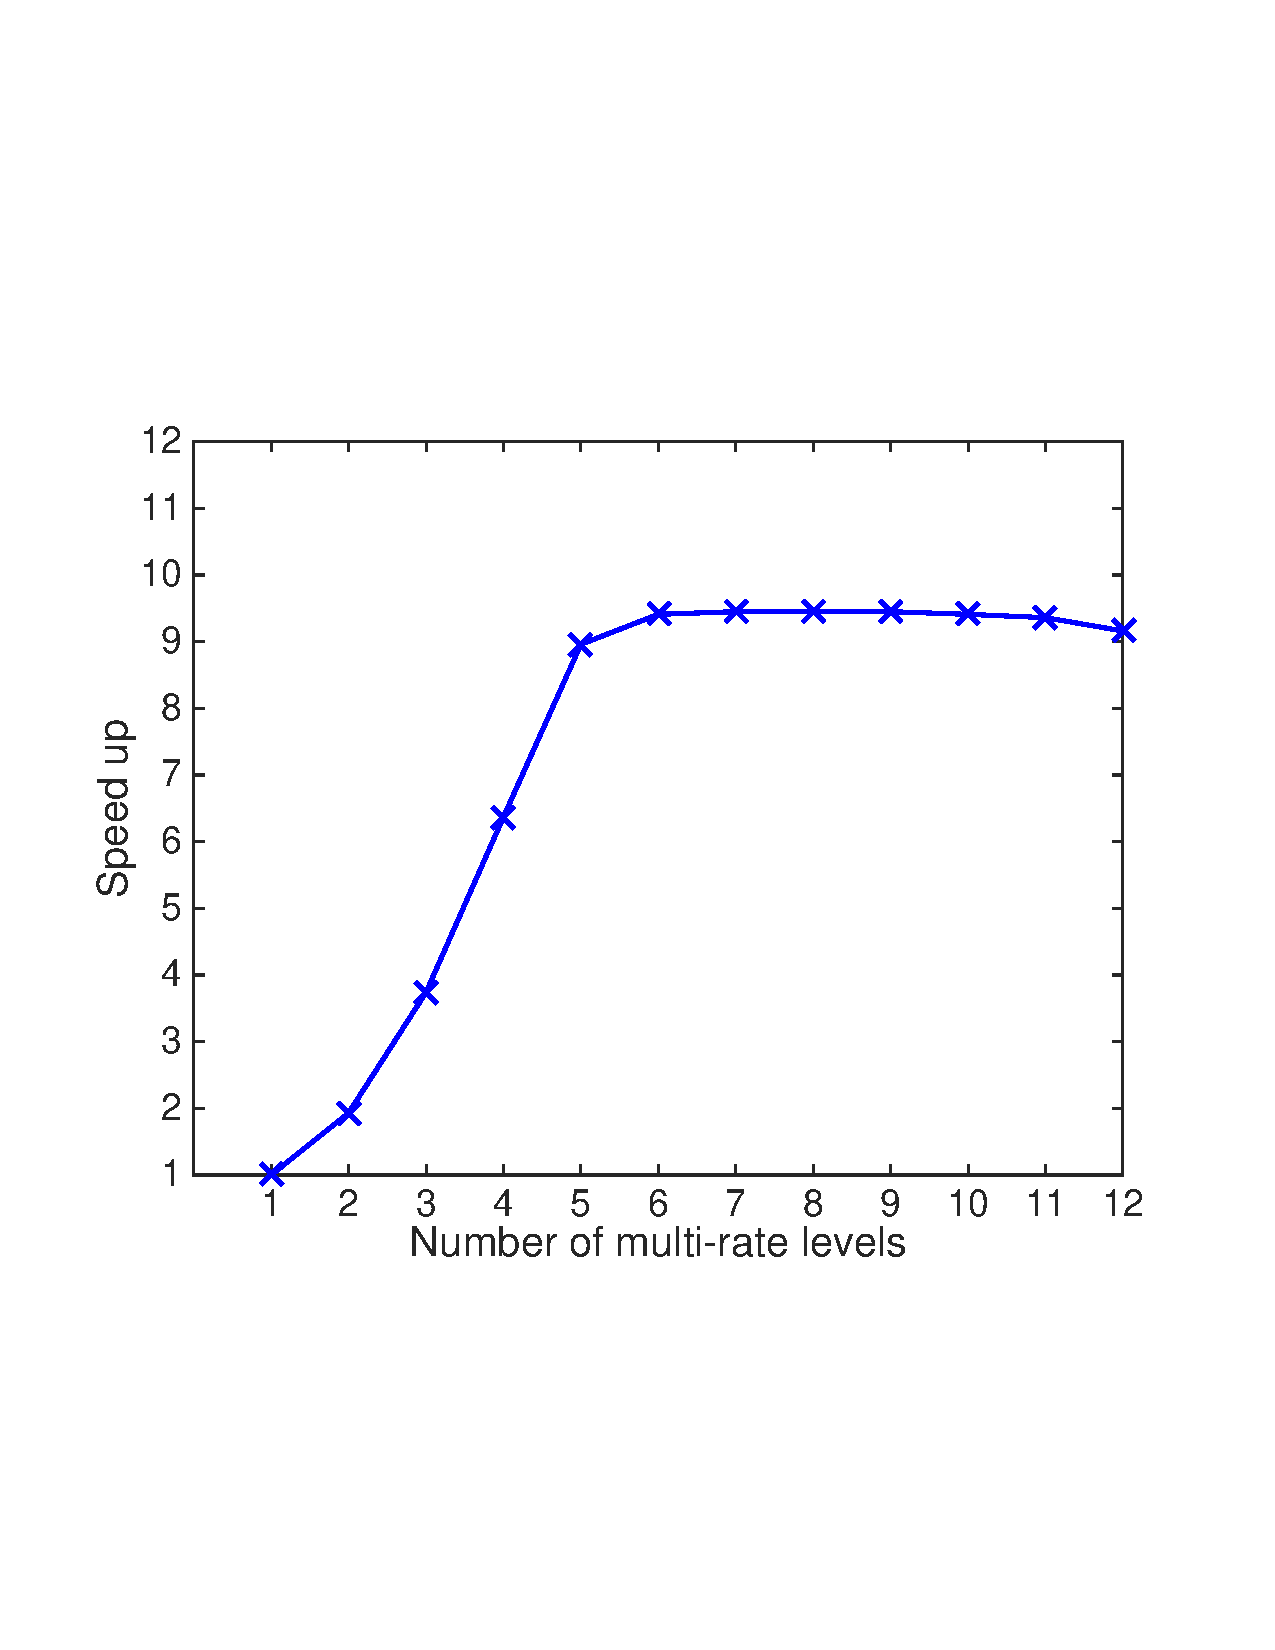
\includegraphics[trim=1cm 6cm 2cm 7cm,clip=true,width=0.5\linewidth]{./figures/timeVsLevelsWorldOcean.pdf}
\caption{\emph{Overall speedup vs the number of multi-rate levels used for the simulation of Japan tsunami in global ocean.}}
\label{fig:timeVsLevelsWorldOcean}
\end{center}
\end{figure}

%Fig (\ref{fig:profile_multirate}) illustrates the percentage of time spent on each level during the simulation. From the Table (\ref{tab:pasidgLevels}), the expected computational cost for $2\%$ of the elements correspond to the finest level is about $6\%$. However,  the computational time spent is more than $10\%$ of the overall time in all the cases. This is because of the under-utilization of the hardware when only fewer elements are processed by a computational kernel.
%\begin{figure}%[h!]
%\begin{center}
%  \subfloat[N=1]{%
%    \begin{minipage}[c]{0.2\linewidth}
%      \centering%
%      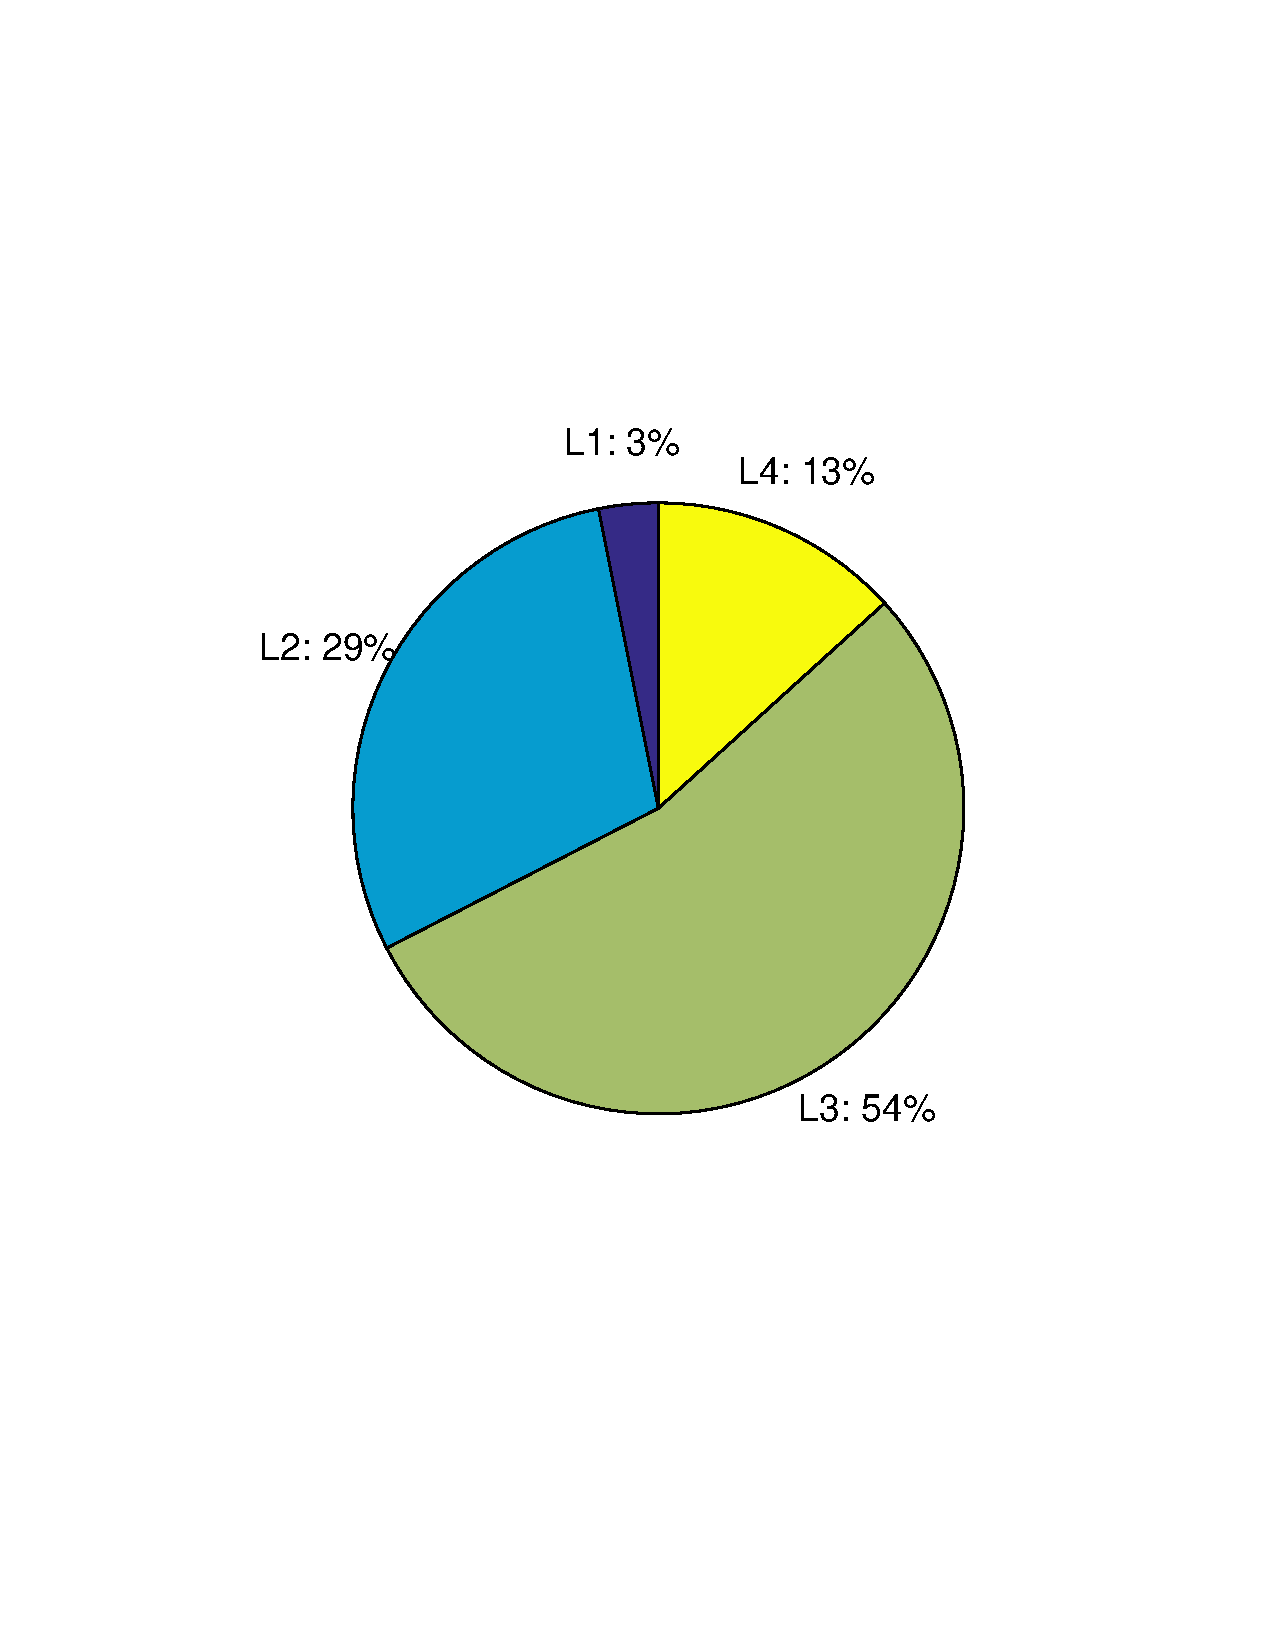
\includegraphics[trim=4cm 8.5cm 2cm 7cm,clip=true,width=\textwidth]{./figures/profileMultirateCudaN1.pdf}
%  \end{minipage}} \hspace{0.3cm}
%  \subfloat[N=2]{%
%    \begin{minipage}[c]{0.2\linewidth}
%      \centering%
%      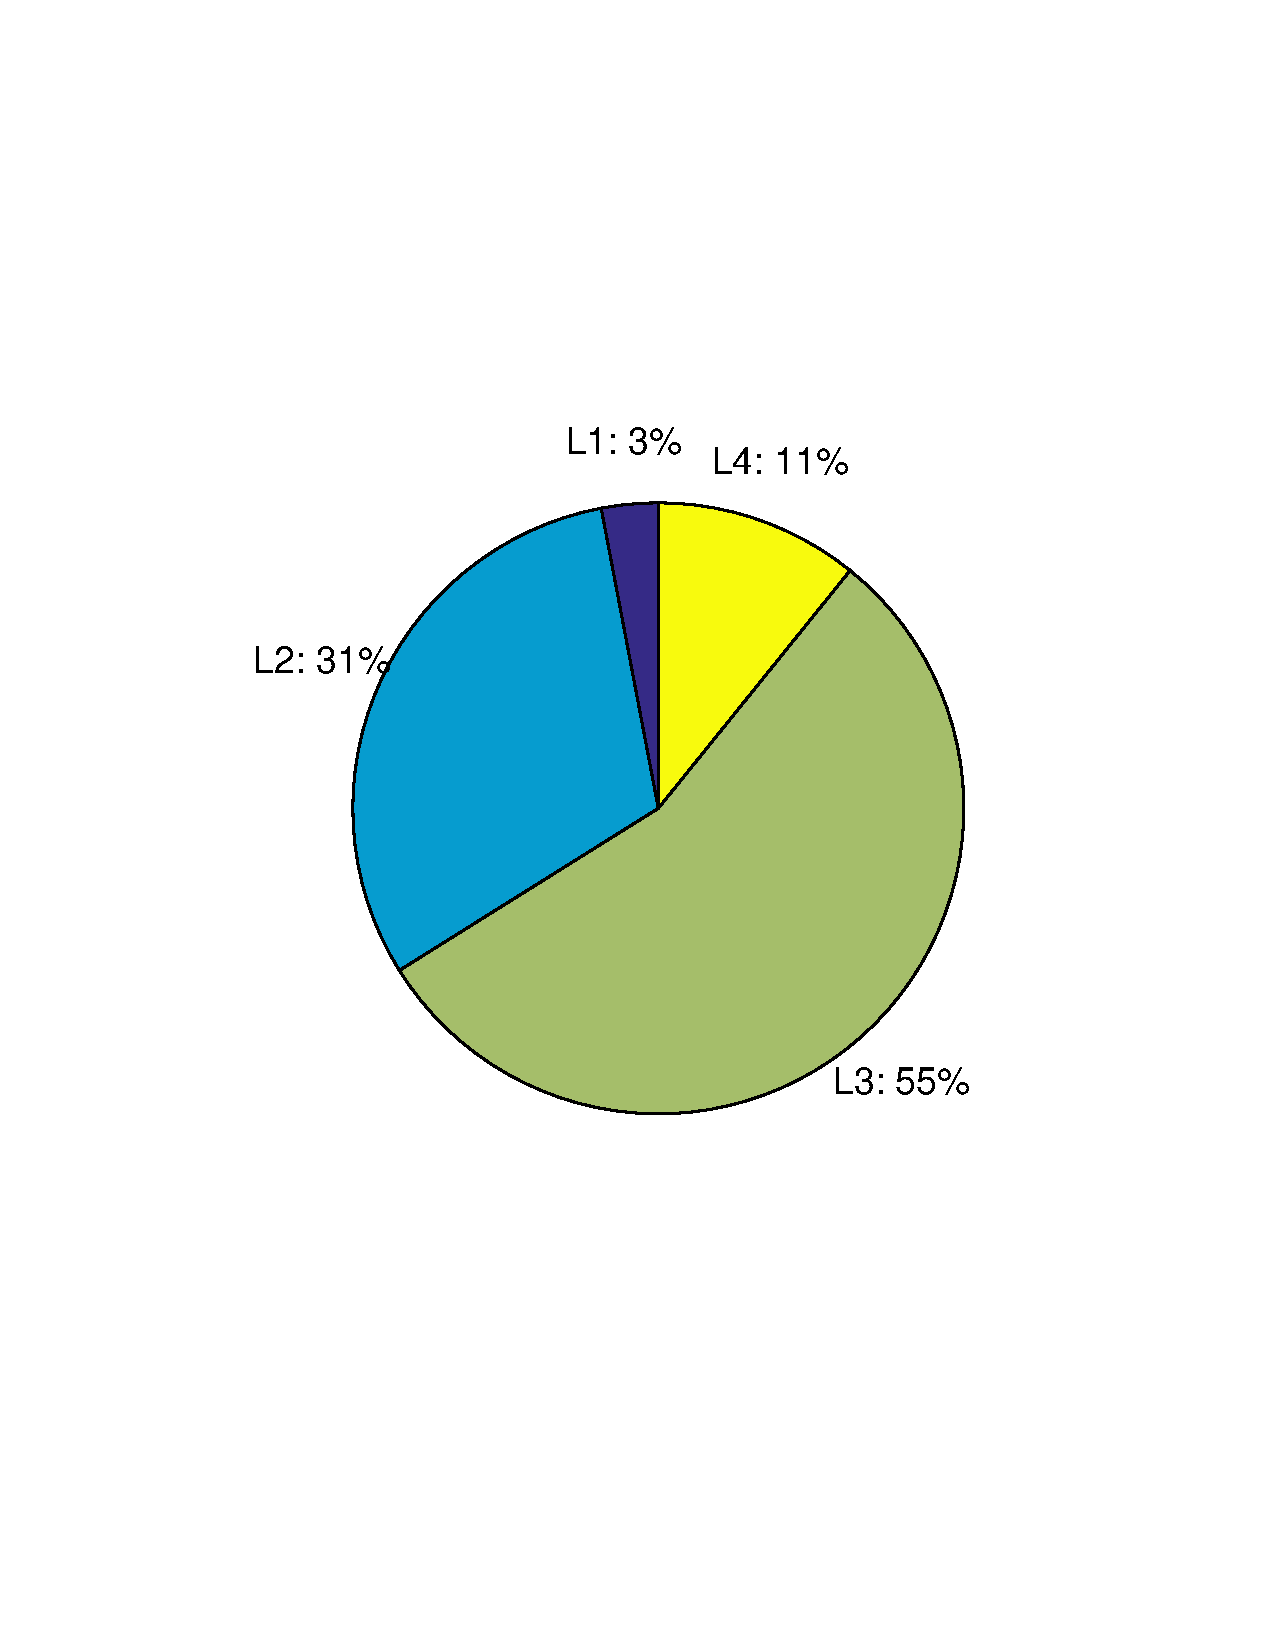
\includegraphics[trim=4cm 8.5cm 2cm 7cm,clip=true,width=\textwidth]{./figures/profileMultirateCudaN2.pdf}
%  \end{minipage}}\hspace{0.3cm}
%    \subfloat[N=3]{%
%    \begin{minipage}[c]{0.2\linewidth}
%      \centering%
 %     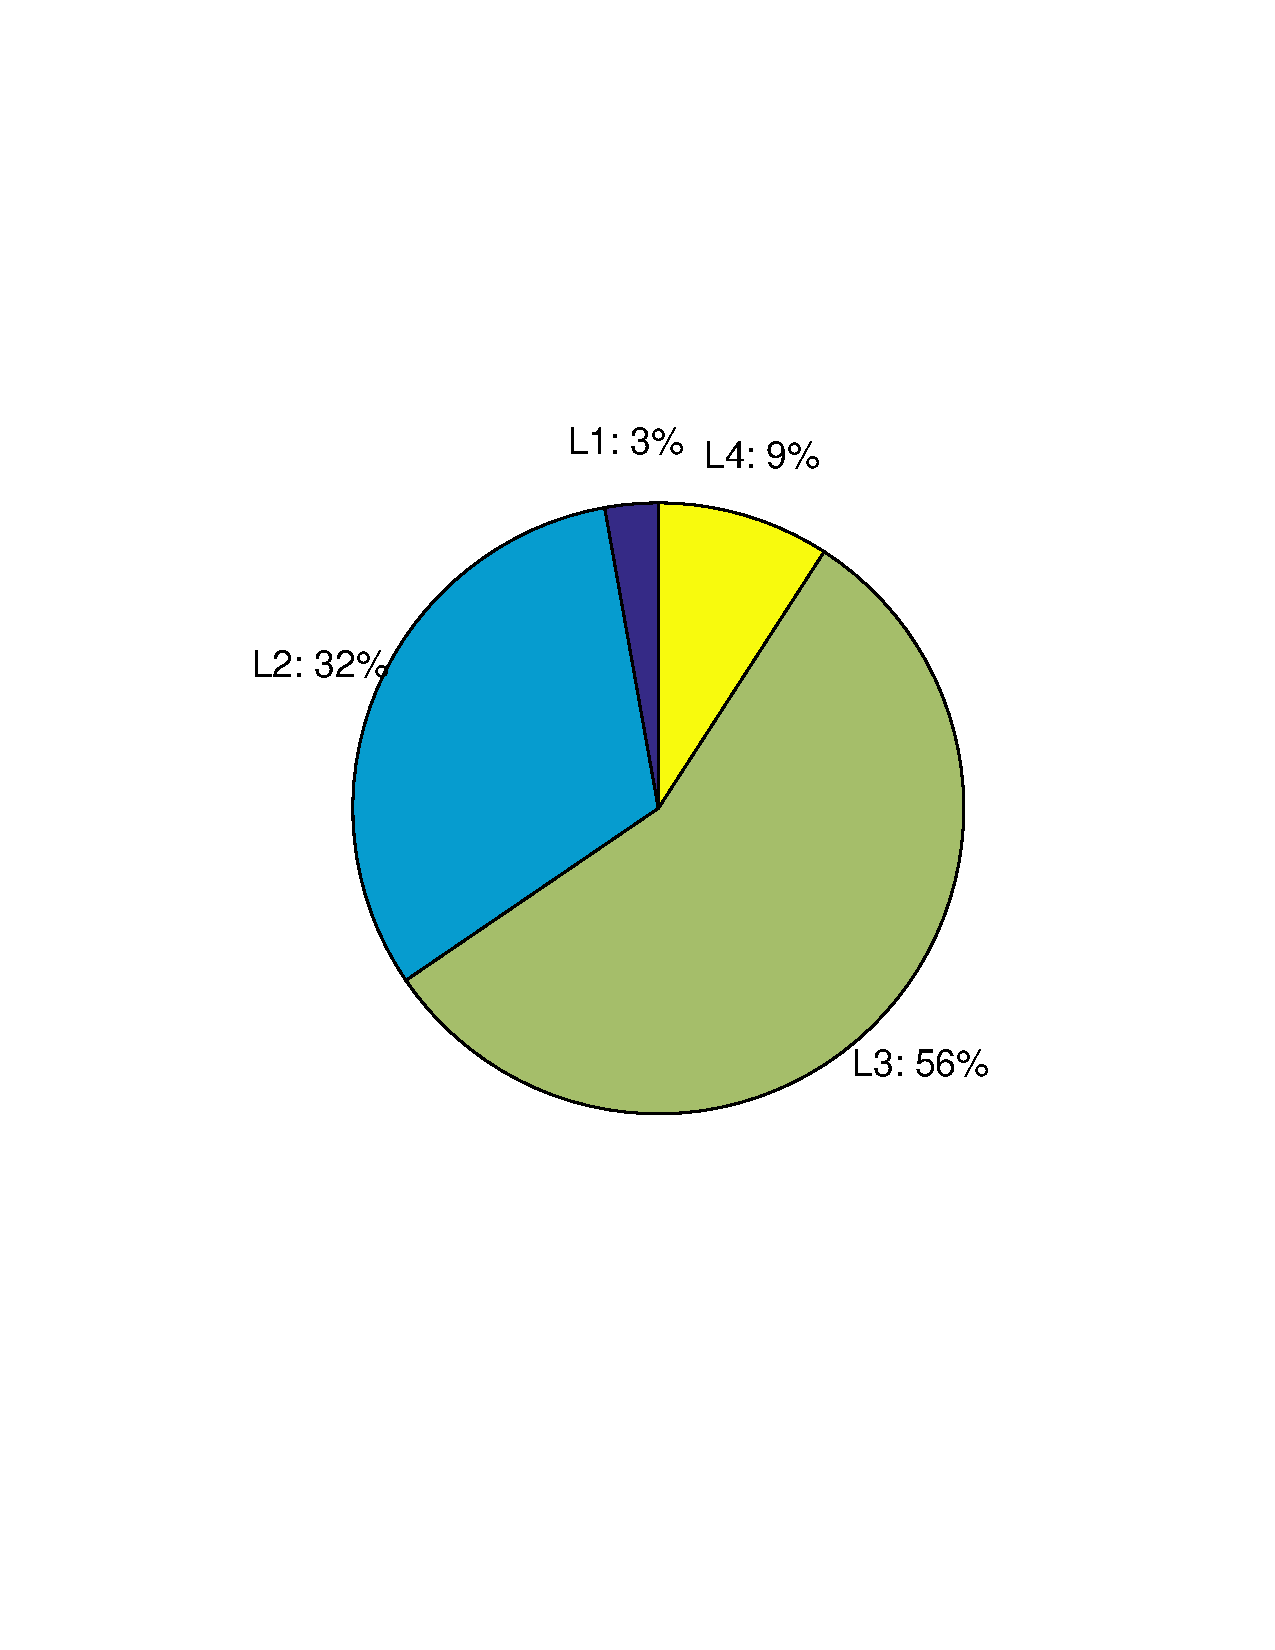
\includegraphics[trim=4cm 8.5cm 2cm 7cm,clip=true,width=\textwidth]{./figures/profileMultirateCudaN3.pdf}
 % \end{minipage}} \hspace{0.3cm}
%  \subfloat[N=4]{%
 %   \begin{minipage}[c]{0.2\linewidth}
 %     \centering%
 %     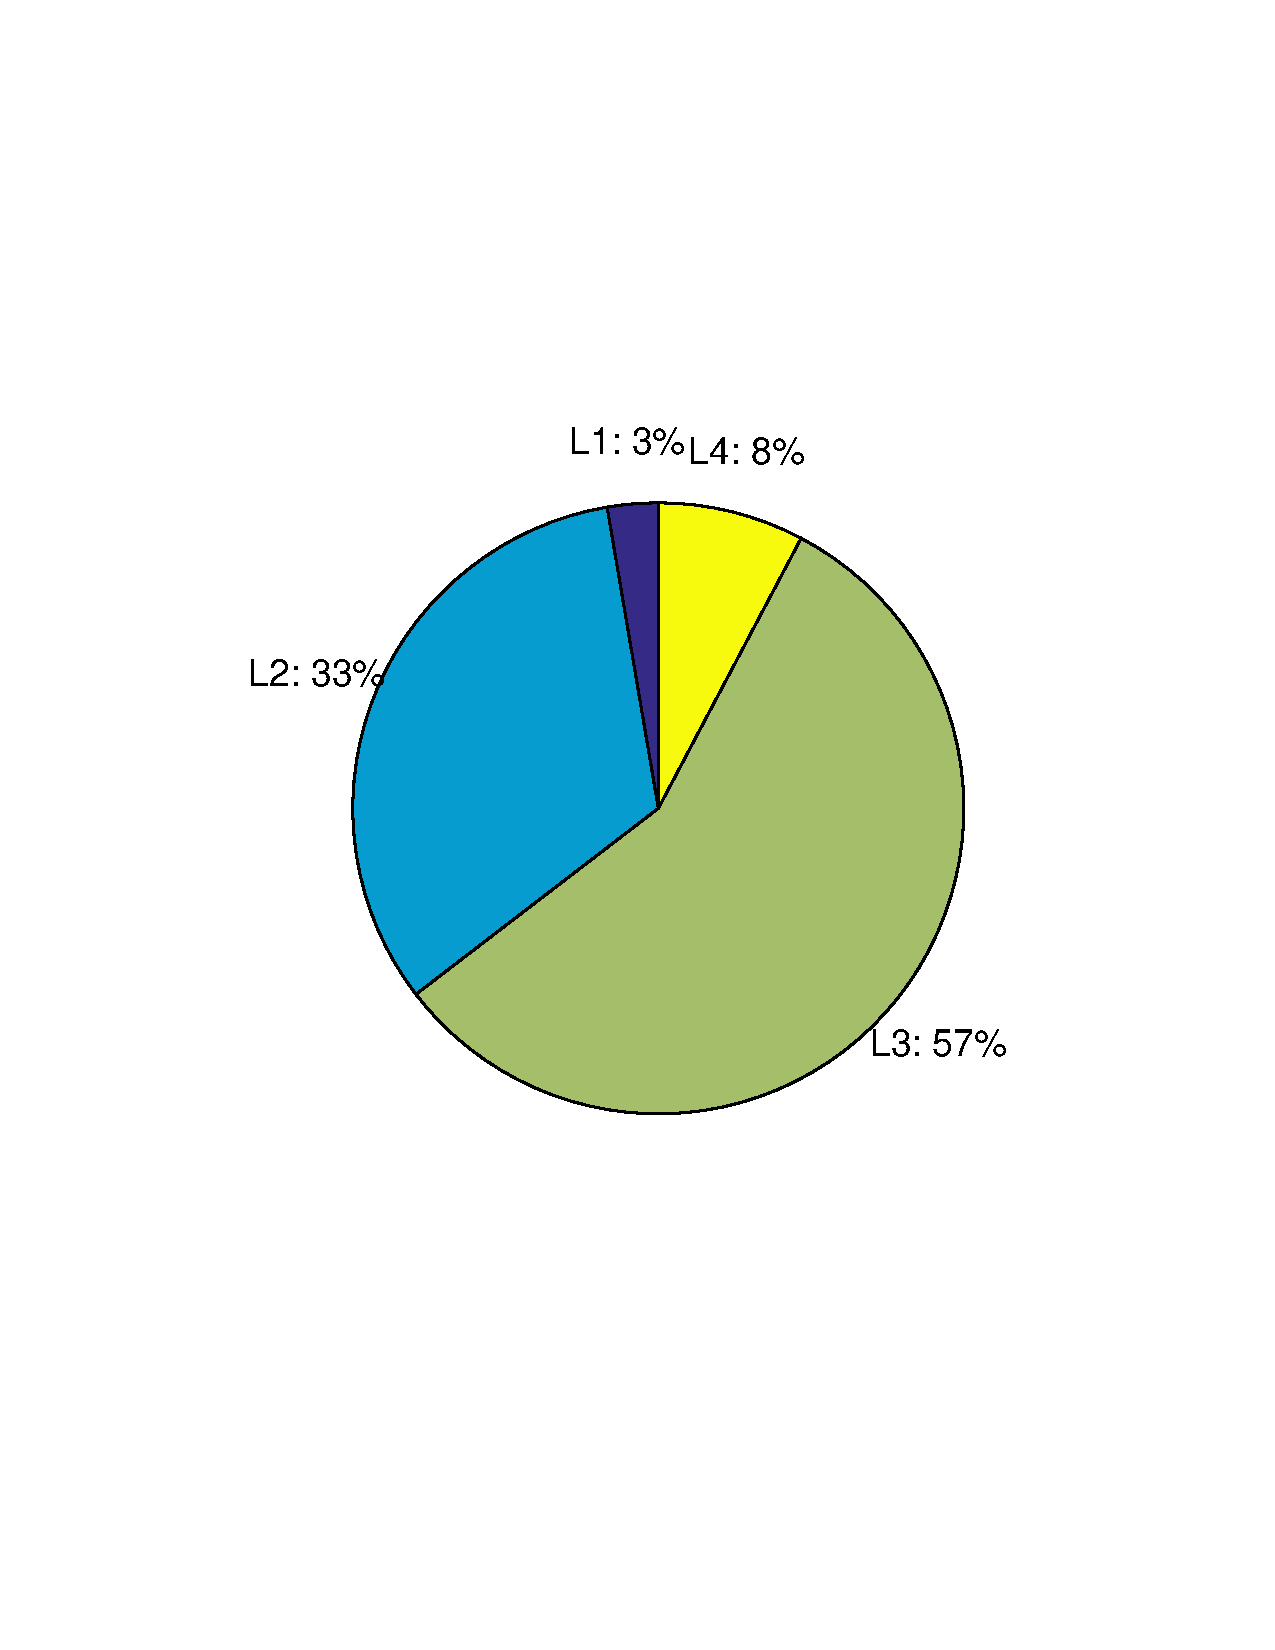
\includegraphics[trim=4cm 8.5cm 2cm 7cm,,clip=true,width=\textwidth]{./figures/profileMultirateCudaN4.pdf}
 % \end{minipage}}
%\end{center}
 %\caption{\emph{Percentage of time spent by each level in the multi-rate time scheme. Simulations are run on one NVIDIA K40c GPU.}}
 % \label{fig:profile_multirate}
%\end{figure}


 The overall computational time for the simulations using polynomial orders $1$, $2$, $3$, and $4$ are given in Tables (\ref{tab:pasidgTiming}, \ref{tab:worldOceanTiming}).  The kernels are tuned using parameters described in \cite{gandham2014swe}. Using CUDA model on NVIDIA K40c GPU, the simulations run as fast as $130$ times the faster than real time with linear polynomials while running at $10$ times faster with $4^{th}$ order polynomials in each triangle, in case of Indian Ocean tsunami.
In these experiments, a single mesh is used for all the discretizations. However, a coarser mesh may provide similar predictions for higher order DG discretizations.
\begin{table}[h!]
\begin{center}
\begin{tabular}{crrr}
\hline
Polynomial & \# unknowns & Compute& Real/  \\
order & (millions)& time (min) & compute\\ \hline
1 & 1.17 &  5 & 130\\
2 & 2.34 & 14 &  41\\
3 & 3.90 & 33 &  18\\
4 & 5.85 & 64 &  10\\\hline
\end{tabular}
\caption{\emph{The overall compute time of 10 hrs of Indian Ocean tsunami simulation using an NVIDIA K40c GPU. The simulation used OCCA:CUDA model and single precision arithmetic.}}
\label{tab:pasidgTiming}
\end{center}
\end{table}

\begin{table}[h!]
\begin{center}
\begin{tabular}{crrr}
\hline
Polynomial & \# unknowns & Compute& Real/  \\
order & (millions)& time (min) & compute\\ \hline
1 & 15.8 &  36 & 16\\
2 & 31.6 & 100 &  6\\
3 & 52.7 & 220 & 2.7\\
4 & 79.1 & 460 & 1.3\\\hline
\end{tabular}
\caption{\emph{The overall compute time of 10 hrs of Japan tsunami simulation using an NVIDIA K40c GPU. 
The simulation used OCCA:CUDA model and single precision arithmetic.}}
\label{tab:worldOceanTiming}
\end{center}
\end{table}
